\chapter{Physics Object and Event Selection}\label{sec:selection}
This chapter outlines the basic \hzg{} physics object and event selection before any event categorization is done.
Along the way, we will also point out the most relevant corrections applied, including trigger scale factors (SFs), physics object energy and momentum corrections, and identification and isolation SFs.

\section{Primary Vertex}
Events are required to have at least one good primary vertex (PV)
with a reconstructed longitudinal position within 24\cm of the
geometric center of the detector and a transverse position within
2\cm of the nominal beam collision point. 
To avoid fake vertices, the PV reconstruction is required to have more than four degrees of freedom.
In the case of multiple satisfactory vertices, the vertex with the highest scalar sum of squared \pt is chosen.

\section{Triggers}
The topology and kinematics of the \hzg{} process guide the choice of triggers used in this analysis. As there are at least three final state decay products, 
the photon \pt tends to be less than in other channels, such as \hgg. Consequently, the CMS single photon trigger \pt thresholds 
are too great to make them viable options. In addition, there is no suitable unprescaled multijet plus photon trigger to target events with 
hadronic decays of the $\PZ$ boson, so the triggers are chosen to target the $\lplm\gamma$ final states.
Therefore, we trigger on the leptons arising from the decay of the Z boson, which tend 
to have larger values of \pt. The best approach to maximize signal efficiency is to use the double lepton triggers. 
The dielectron trigger requires a leading (subleading) electron with
$\pt > 23\,(12)\GeV$, while the dimuon trigger requires a muon with $\pt > 17\,(8)\GeV$. Events passing both the double muon and double electron triggers are classified as $\mpmm\gamma$ events.

The triggers are applied to both data and simulation. Trigger efficiencies and SFs are measured using the 
simulation samples corresponding to each data-taking year. These measurements use a tag and probe method. 
This method takes advantage of the high purity of $\PZ\to\lplm$ events near the $\PZ$ boson mass peak. 
One lepton functions as the tag, and satisfies a set of tight trigger, identification, isolation, and \pt requirements. 
The second lepton, the probe, must pass a looser selection and is used to measure the efficiency in question. 
Using this approach, trigger efficiencies for each leg of a given double lepton trigger are measured in both data and simulation. 
Then a corrective SF, defined as the ratio of data efficiency to simulation efficiency, is applied to the simulation. 
Scale factors are measured and applied in bins of \pt and $|\eta|$.

For the double electron trigger efficiency measurements, the tag electron must satisfy a set of requirements. The tag must pass 
the single electron trigger, pass a tight cut-based identification, have $\pt>30\,(35)\GeV$ in 2016 (2017 and 2018), and have $|\eta|<2.5$. 
The probe electron must pass a loose electron MVA identification requirement. The details of the electron MVA identification will be described later in this chapter.
The efficiencies for each leg 
of the trigger are measured separately, so in each case, the probe electron must match the trigger leg being measured. 
The efficiencies for each double electron trigger leg for 2016, 2017, and 2018 are shown in Fig. \ref{fig:ele_trig_SF}.
On average, the double electron trigger efficiency is measured to be in the range of 86--97\%, depending on the electron \pt and $\eta$.

\begin{figure}[tb]
	\begin{center}
		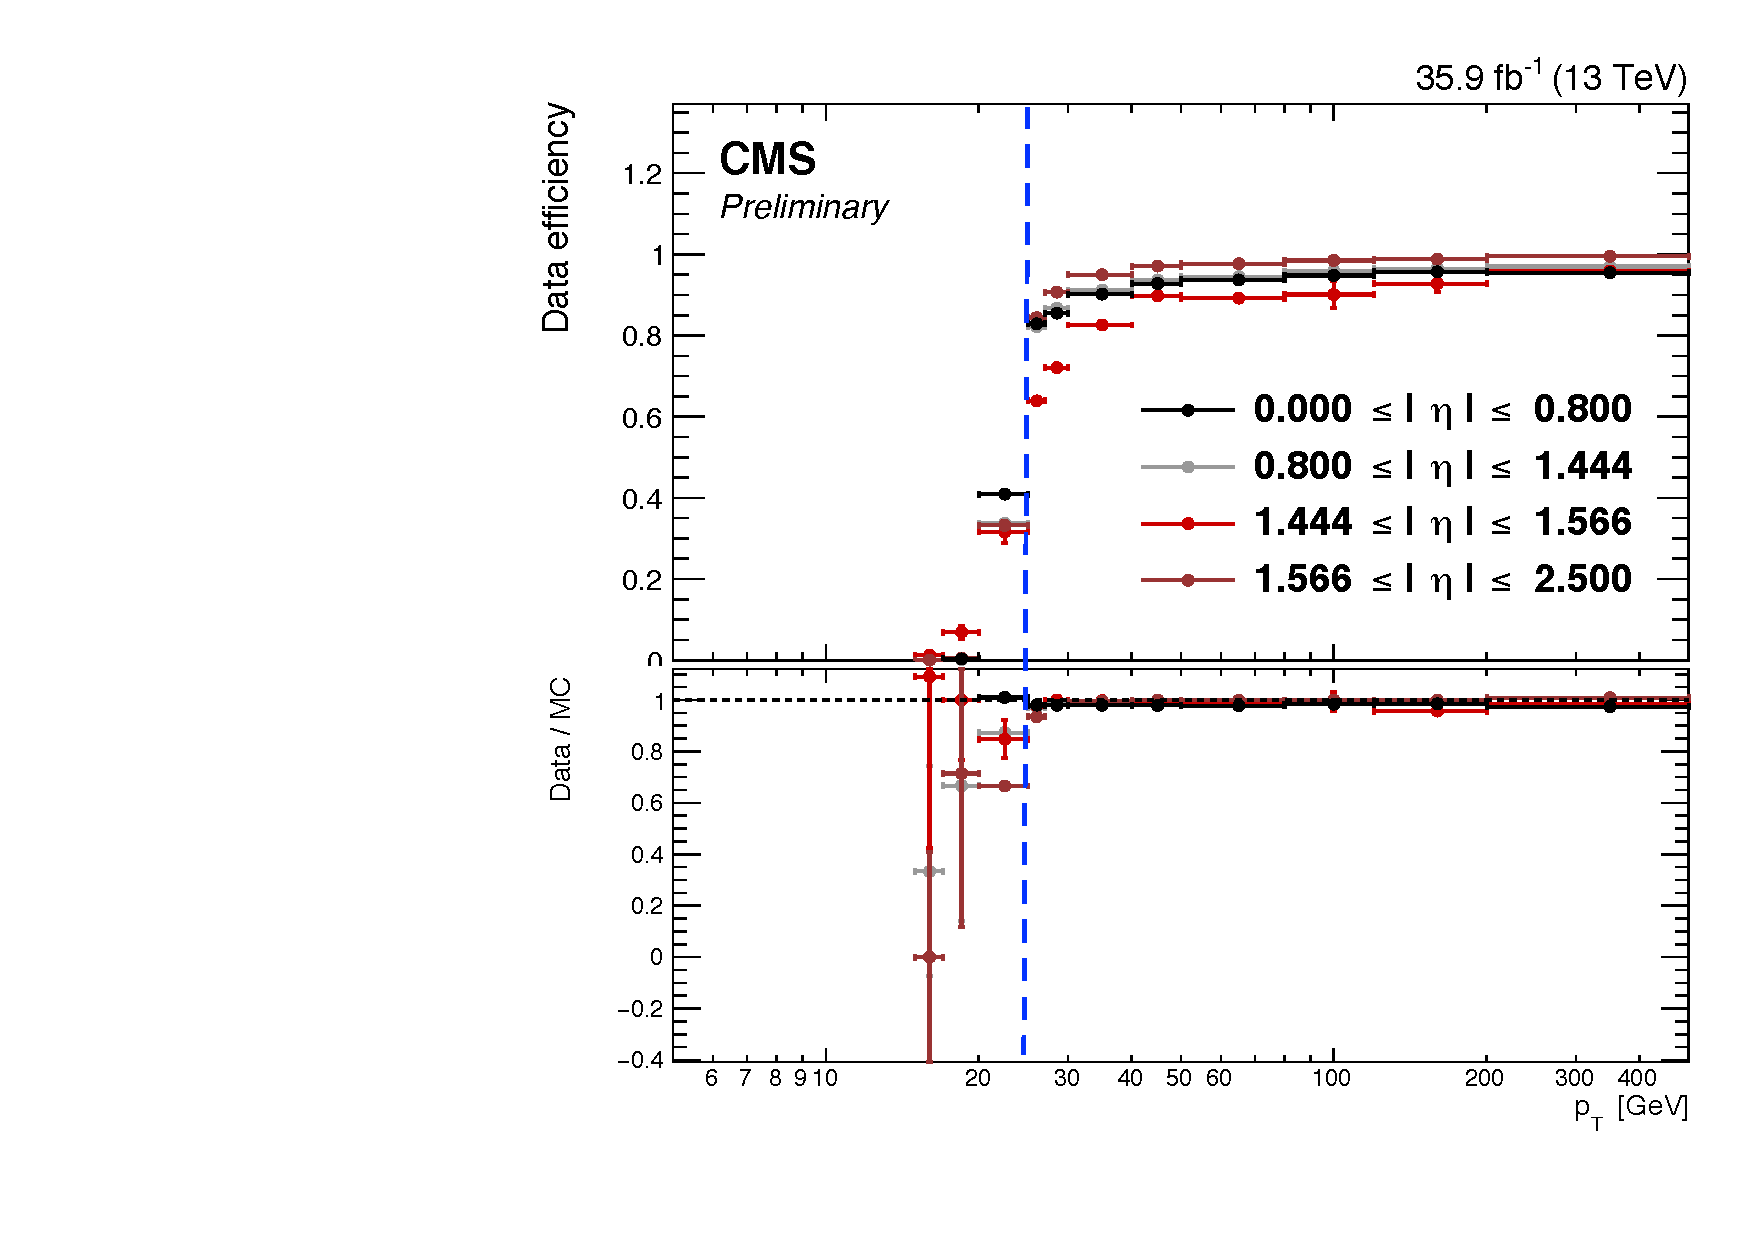
\includegraphics[width=0.30\textwidth]{fig/SFs/2016_ele_trg1_1D.pdf}
		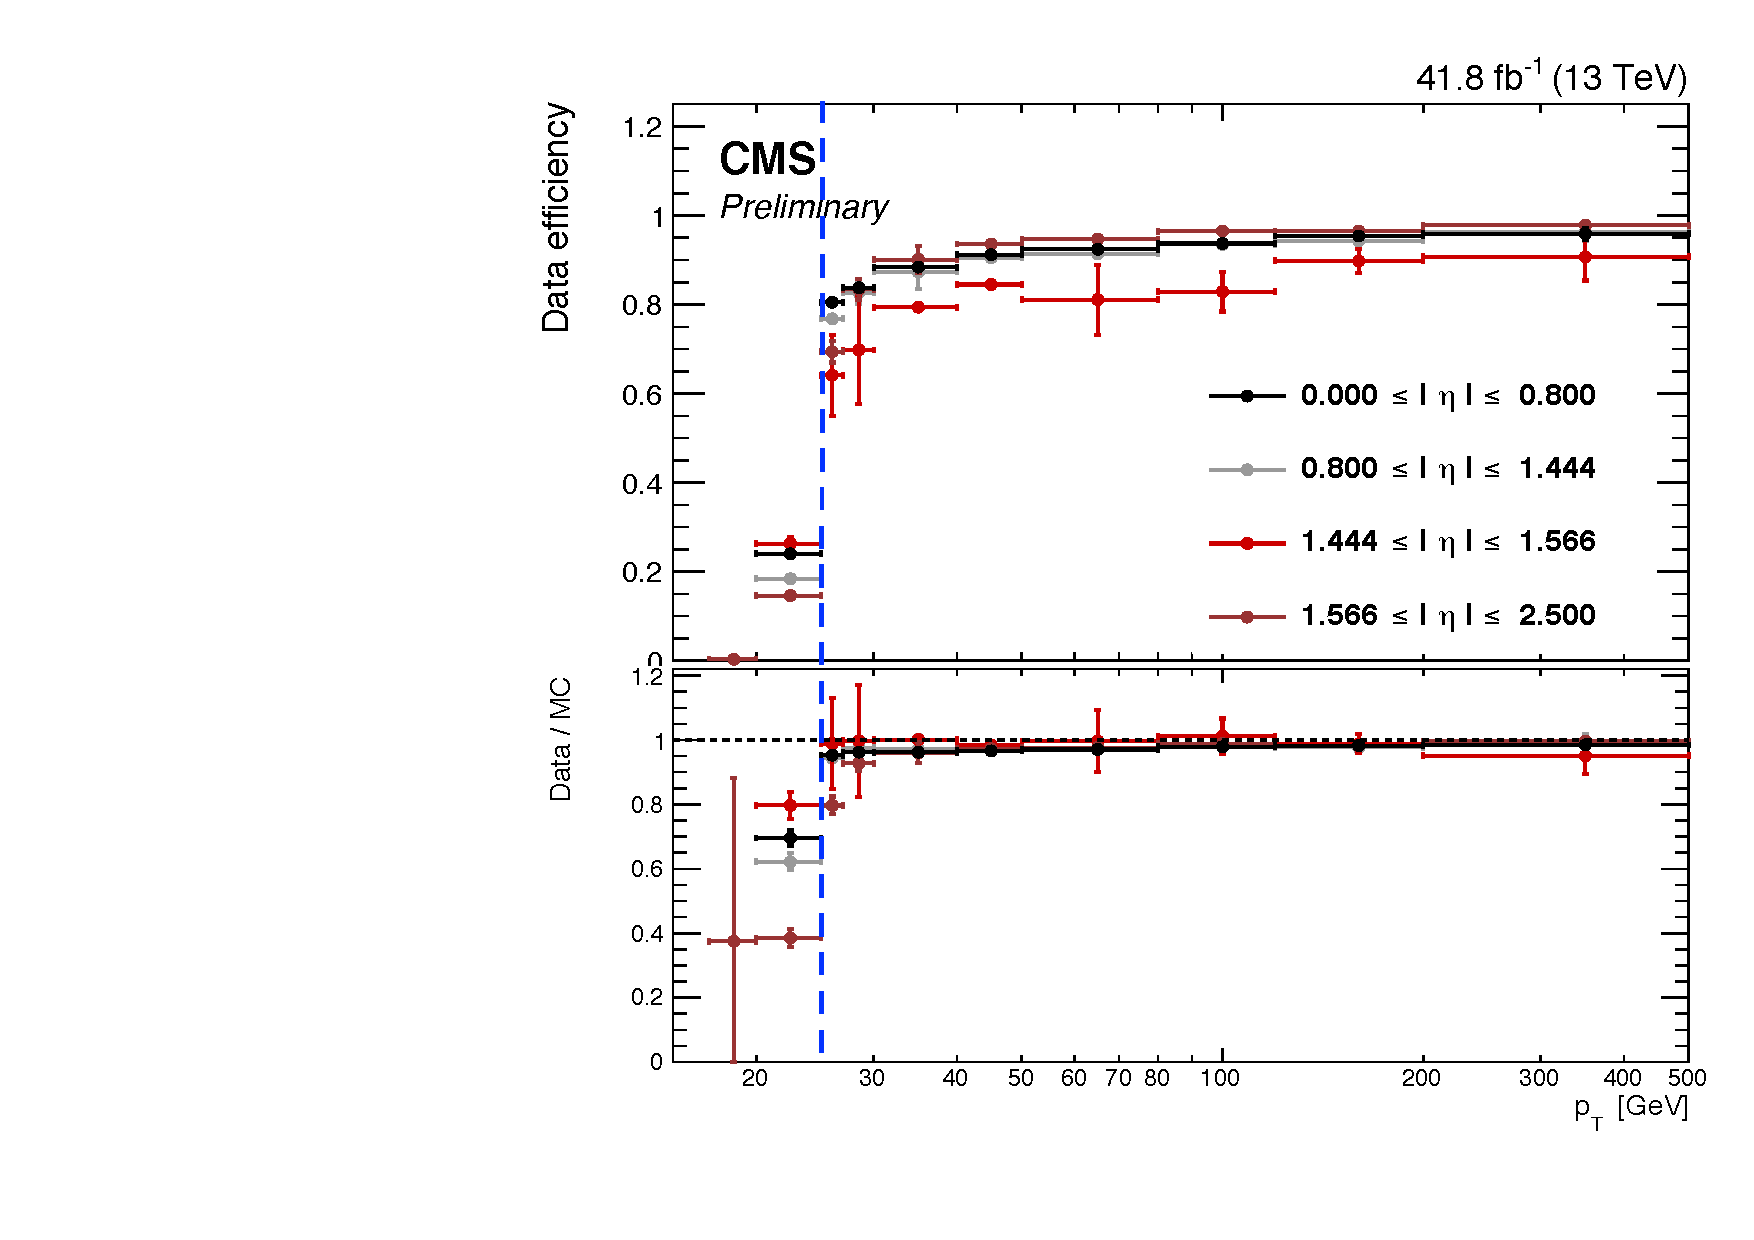
\includegraphics[width=0.30\textwidth]{fig/SFs/2017_ele_trg1_1D.pdf}
		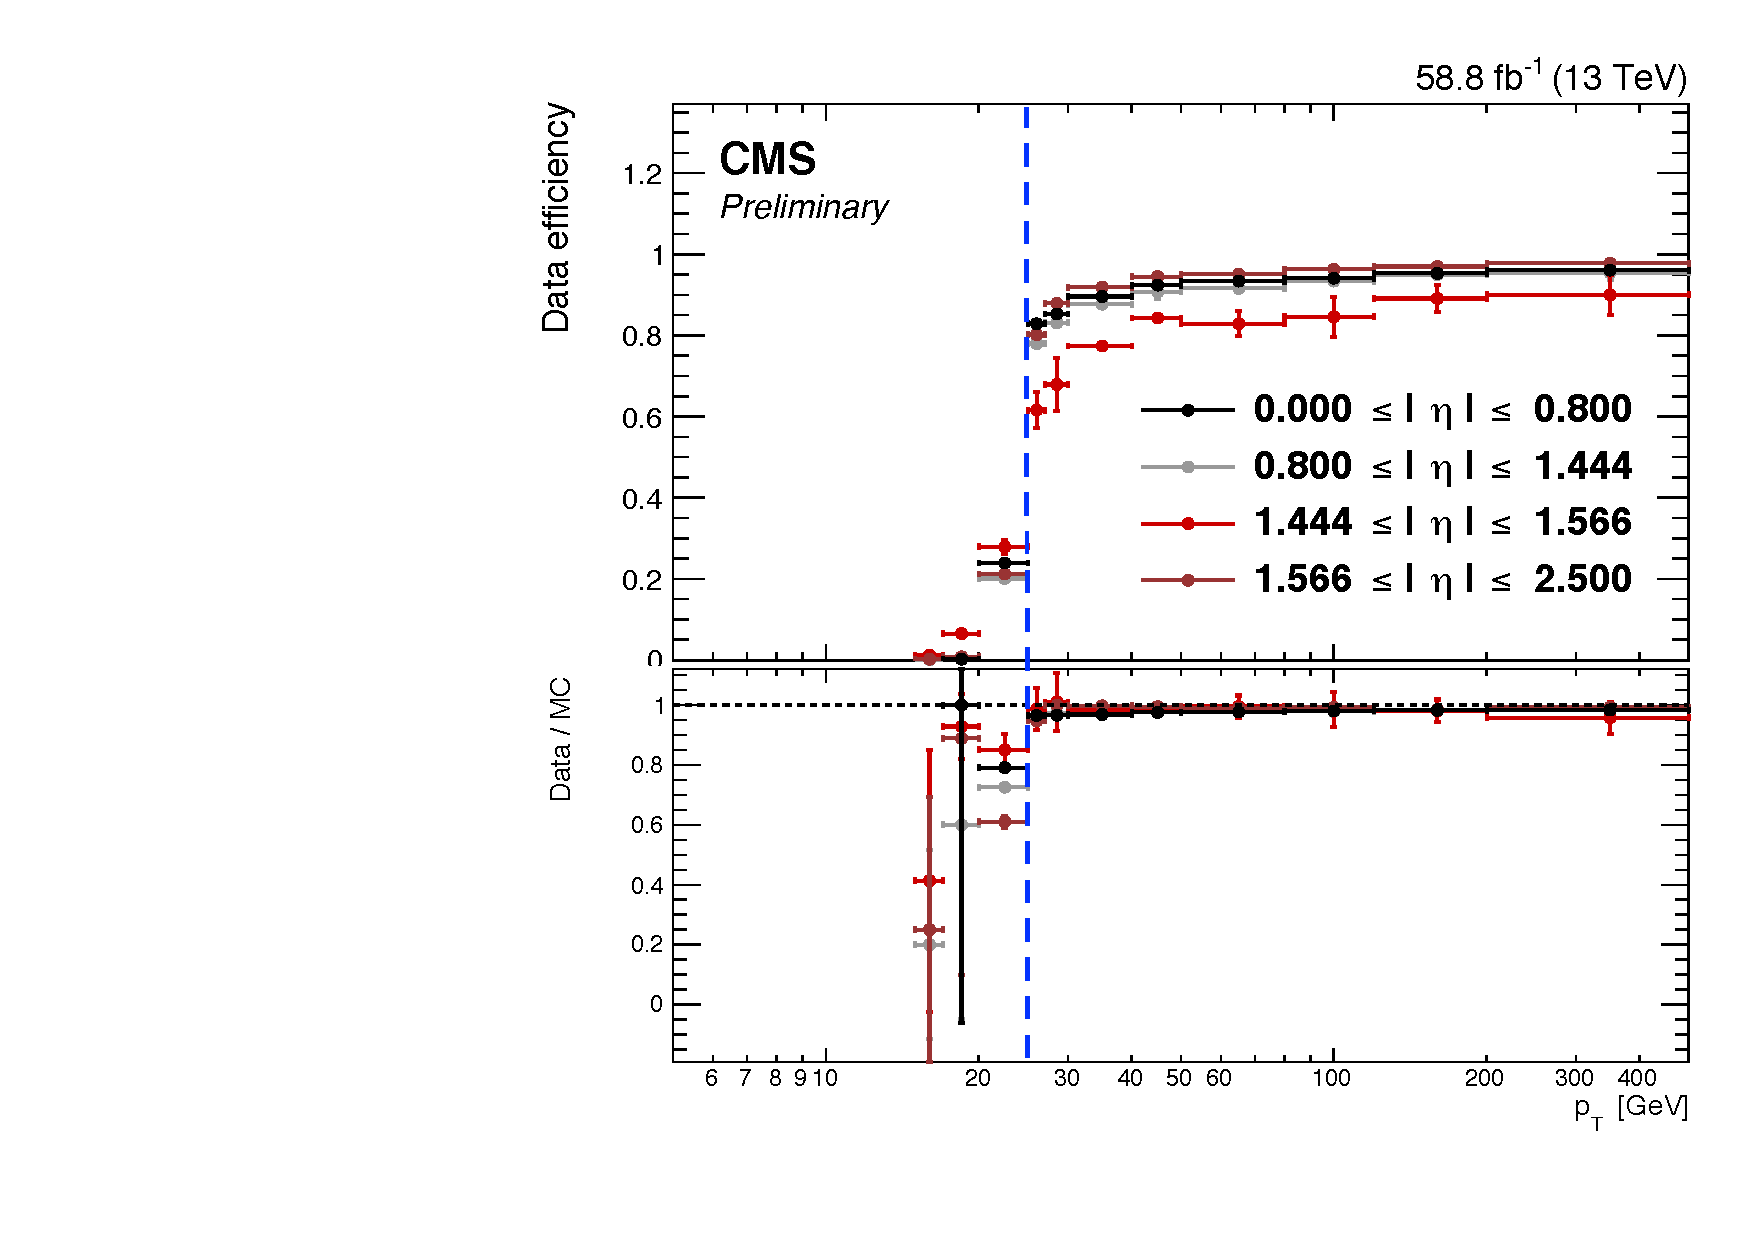
\includegraphics[width=0.30\textwidth]{fig/SFs/2018_ele_trg1_1D.pdf}
		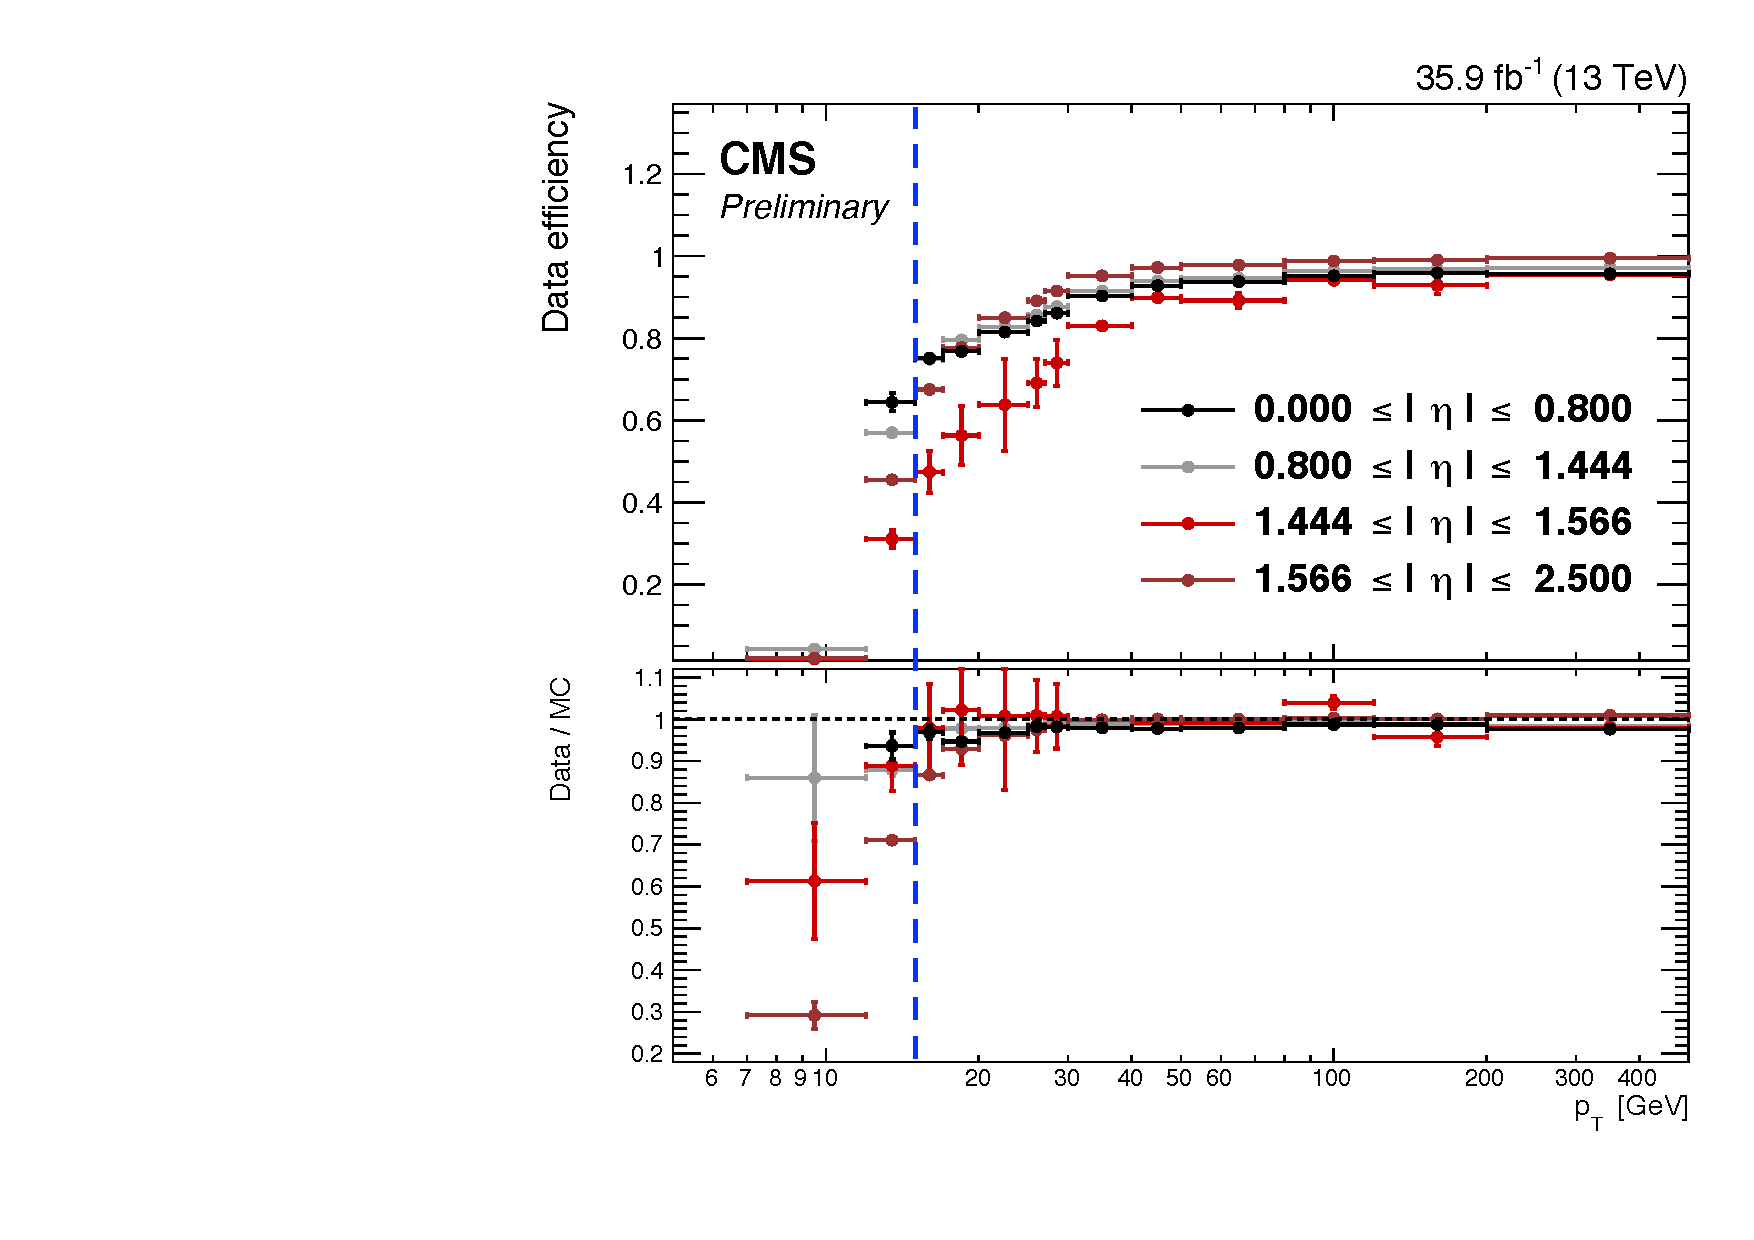
\includegraphics[width=0.30\textwidth]{fig/SFs/2016_ele_trg2_1D.pdf}
		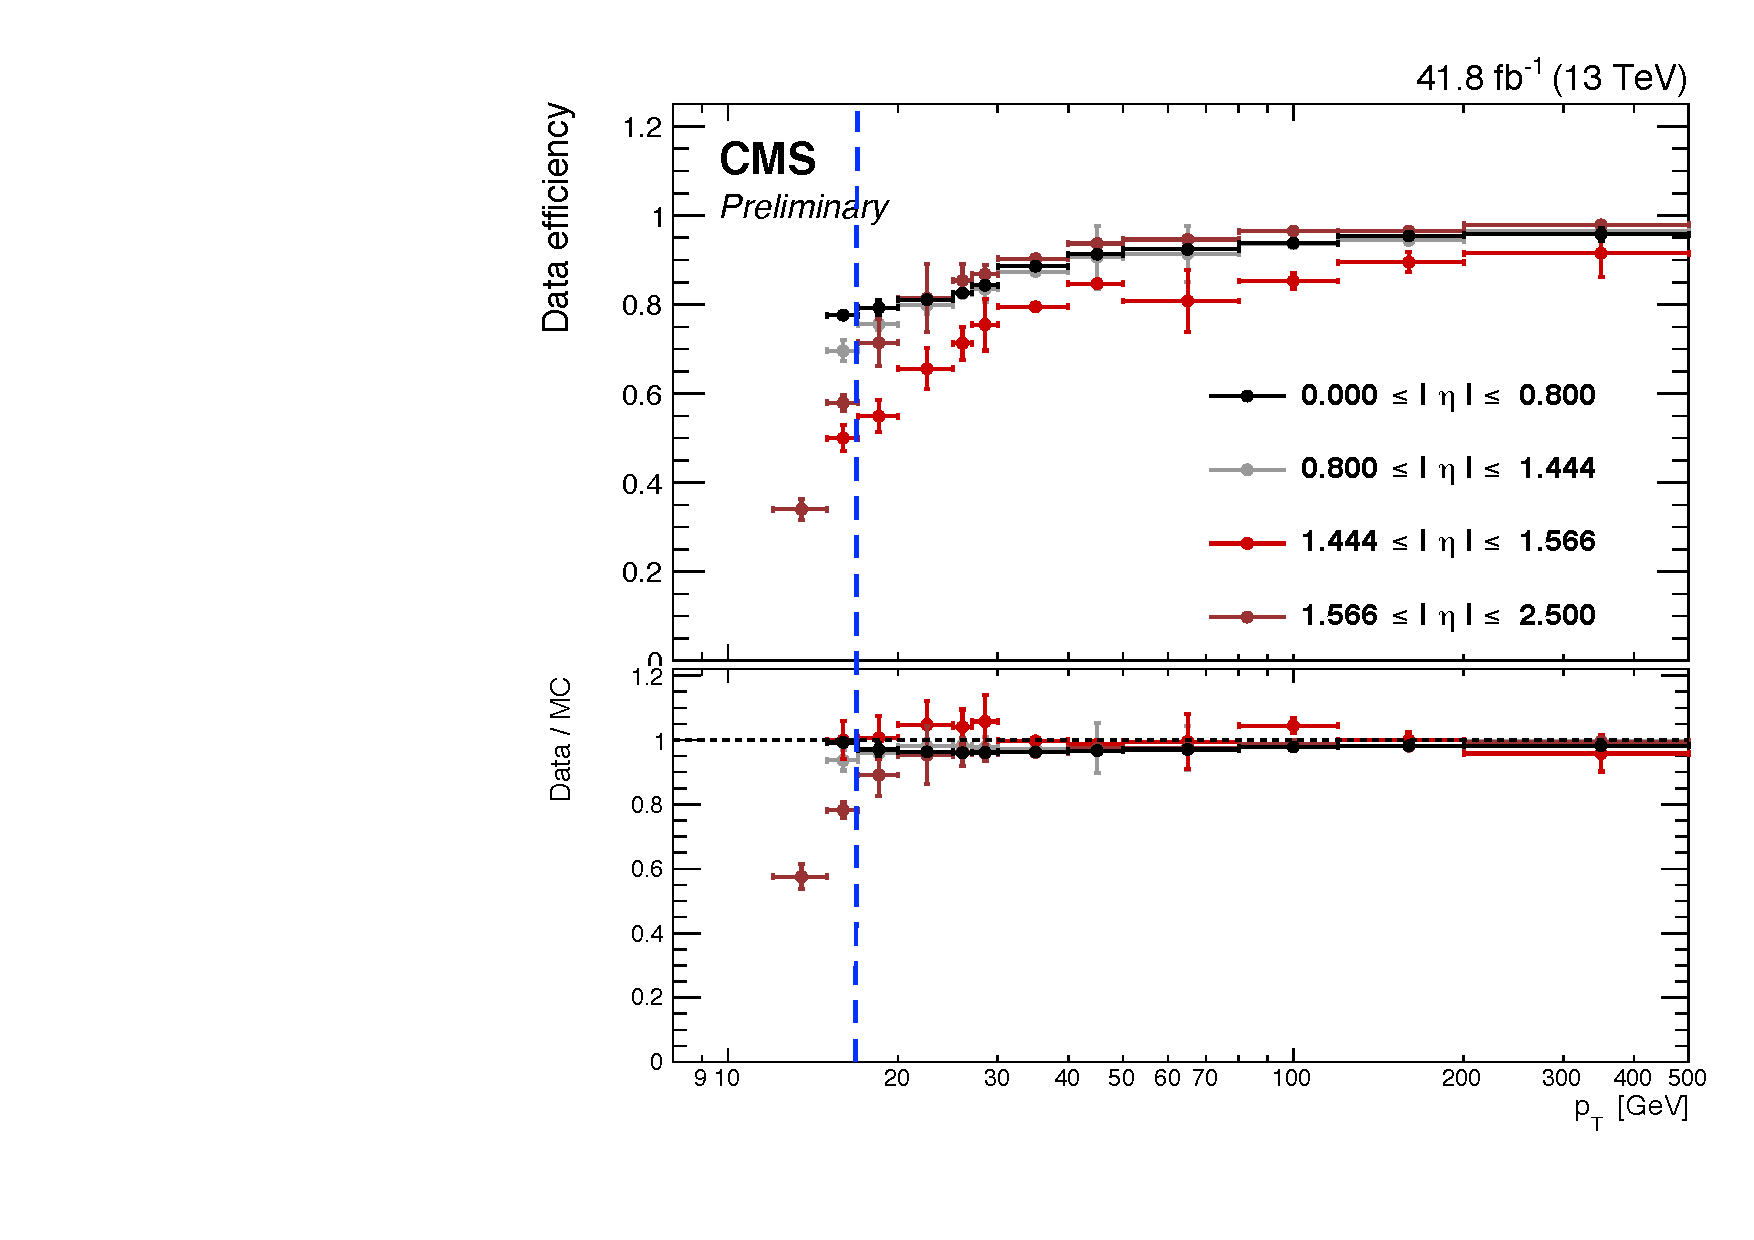
\includegraphics[width=0.30\textwidth]{fig/SFs/2017_ele_trg2_1D.pdf}
		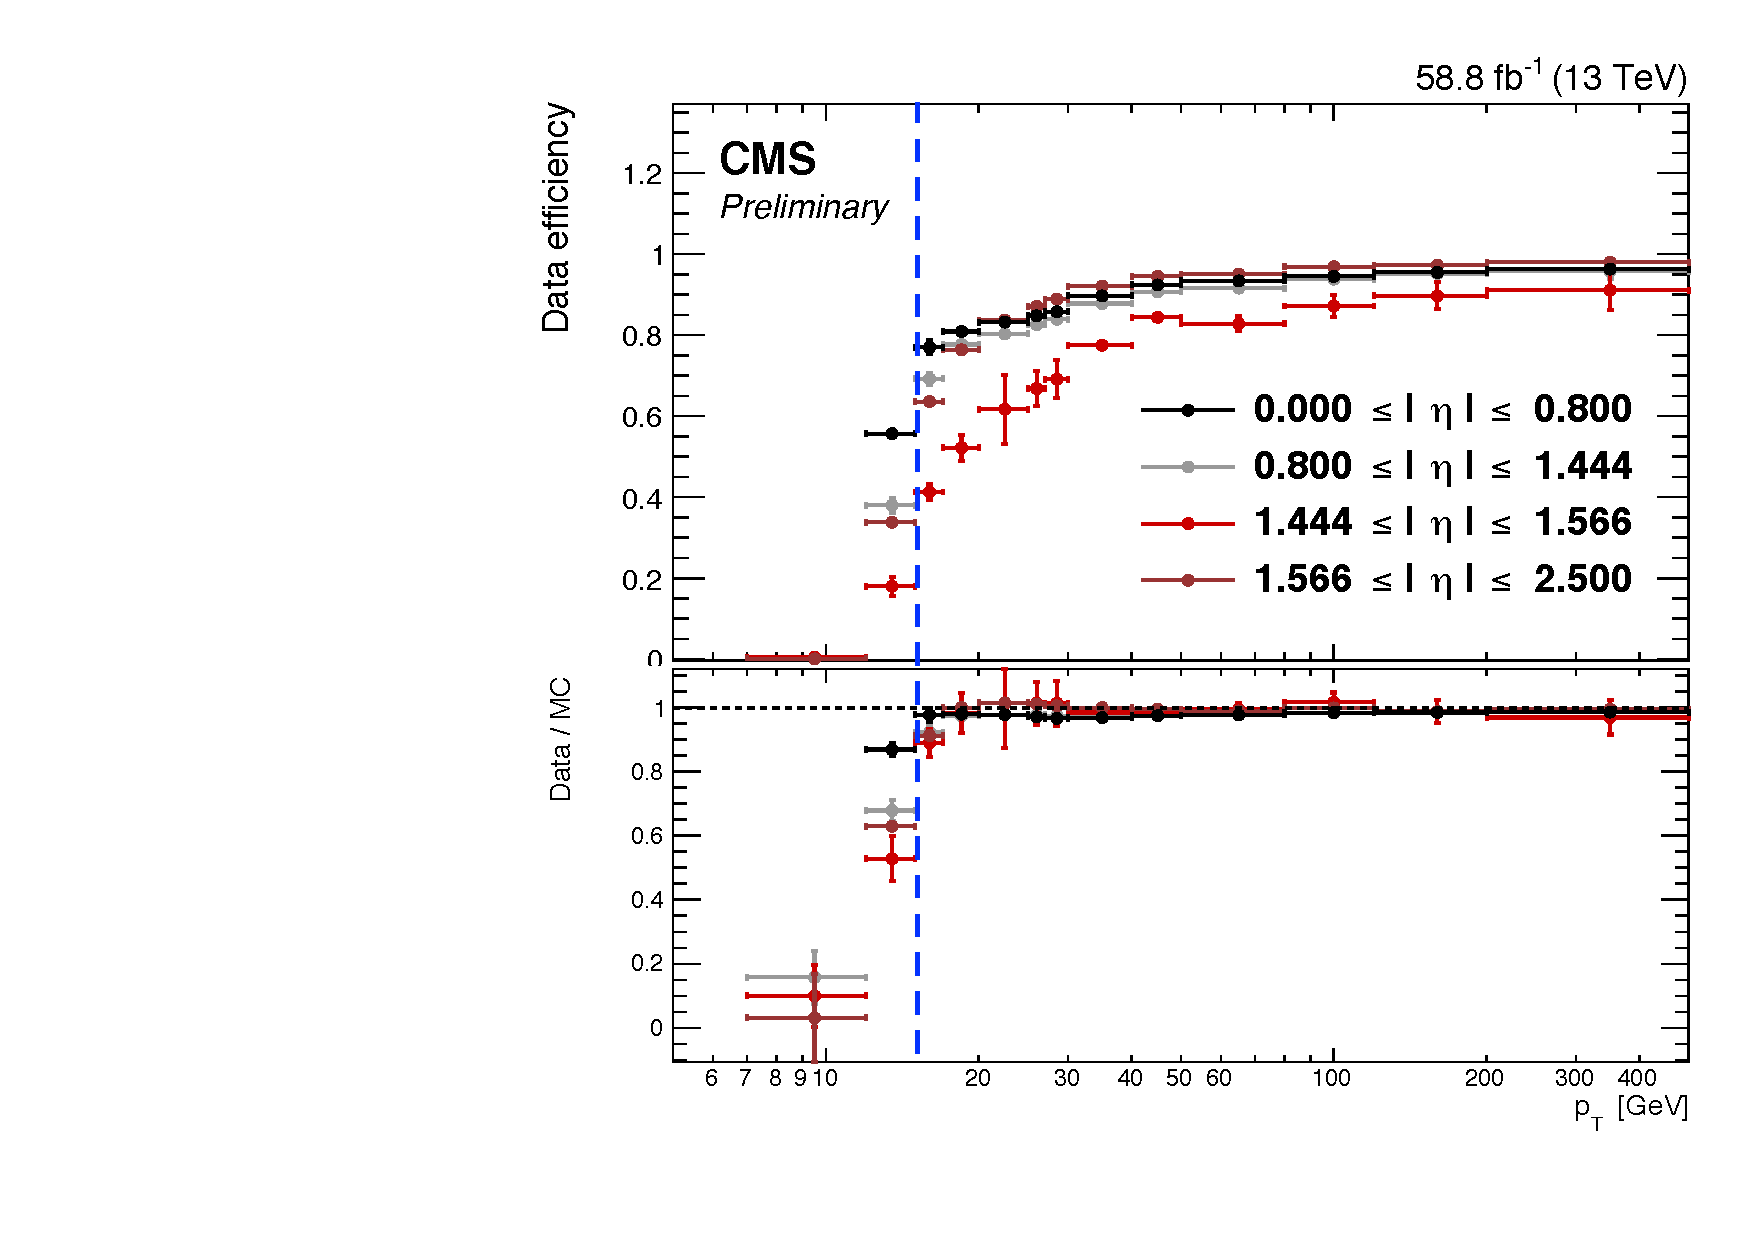
\includegraphics[width=0.30\textwidth]{fig/SFs/2018_ele_trg2_1D.pdf}
	\end{center}
	\caption{Efficiency measurements for each leg of the double electron trigger in 2016 (left), 2017 (center), and 2018 (right). The upper (lower) plots correspond to the 
	leading (subleading) trigger leg.}
	\label{fig:ele_trig_SF}
\end{figure}

For the double muon trigger efficiency measurements, the tag muon must satisfy a set of requirements. It must pass the single 
muon trigger, pass a tight cut-based identification, have $\pt>26\,(29)$ GeV for 2016 (2017 and 2018) and satisfy $|\eta| < 2.4$. The 
probe muon must pass the $\PH\to\PZ\PZ$ identification and isolation cuts. The details of the $\PH\to\PZ\PZ$ muon 
identification will be described later in this chapter. The efficiencies for each leg of the trigger are measured separately, so in each case, the probe 
muon must match the trigger leg being measured. The efficiencies for each double muon trigger leg for 2016, 2017, 
and 2018 are shown in Fig. \ref{fig:mu_trig_SF}. On average, the double muon trigger efficiency is measured to be in the range of 93--95\%, depending on the muon \pt and $\eta$.

\begin{figure}[tb]
	\begin{center}
		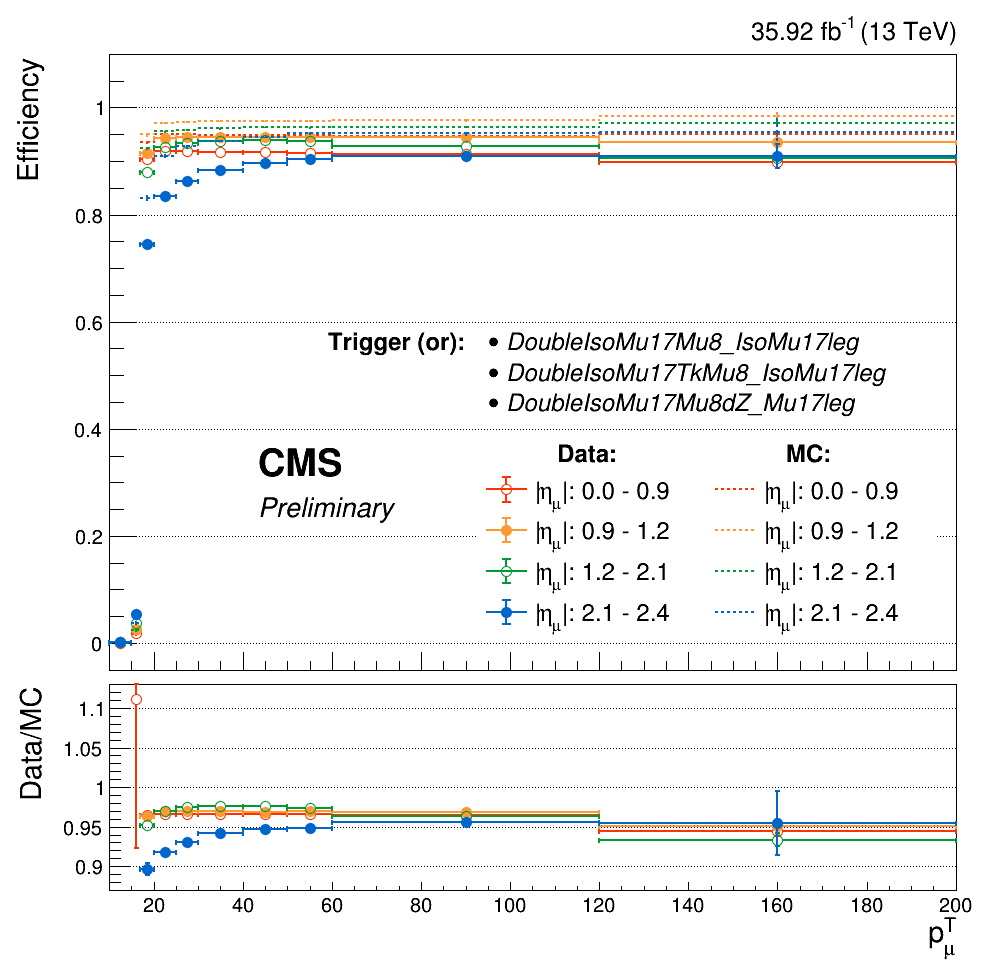
\includegraphics[width=0.30\textwidth]{fig/SFs/sf1D_year2016_leg1.png}
		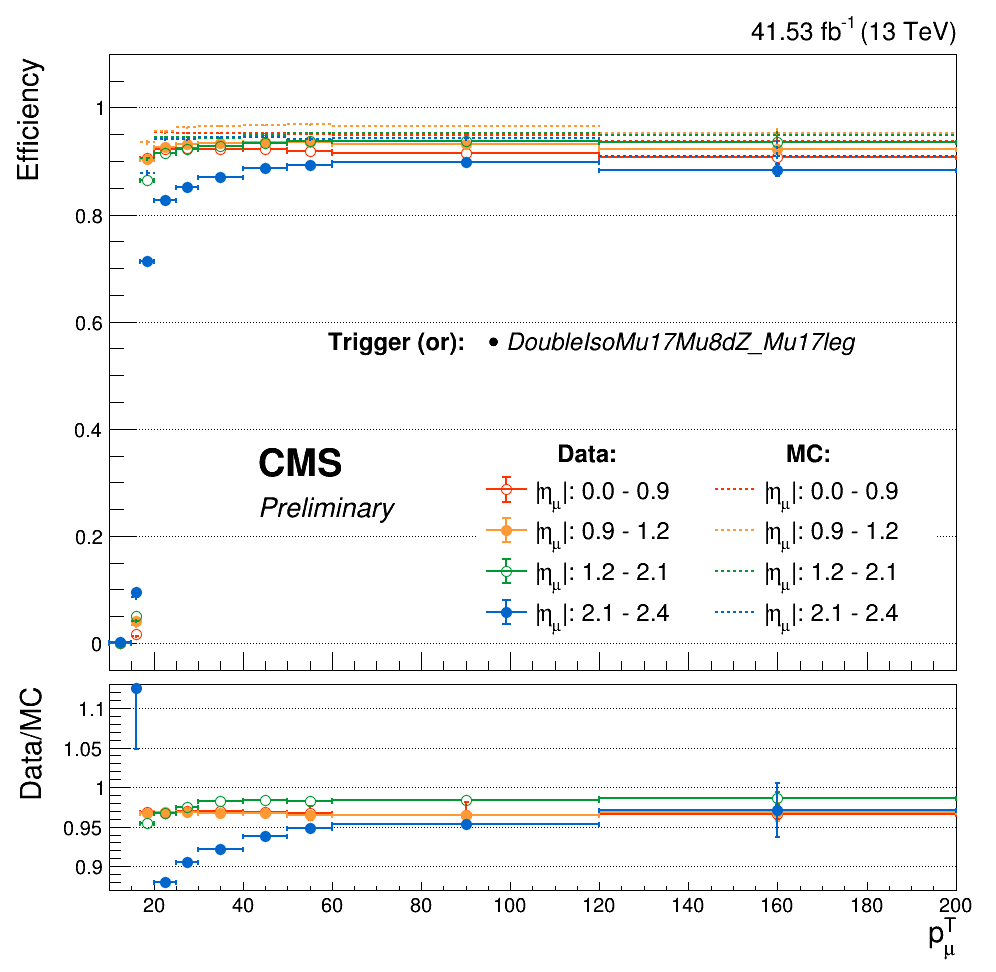
\includegraphics[width=0.30\textwidth]{fig/SFs/sf1D_year2017_leg1.png}
		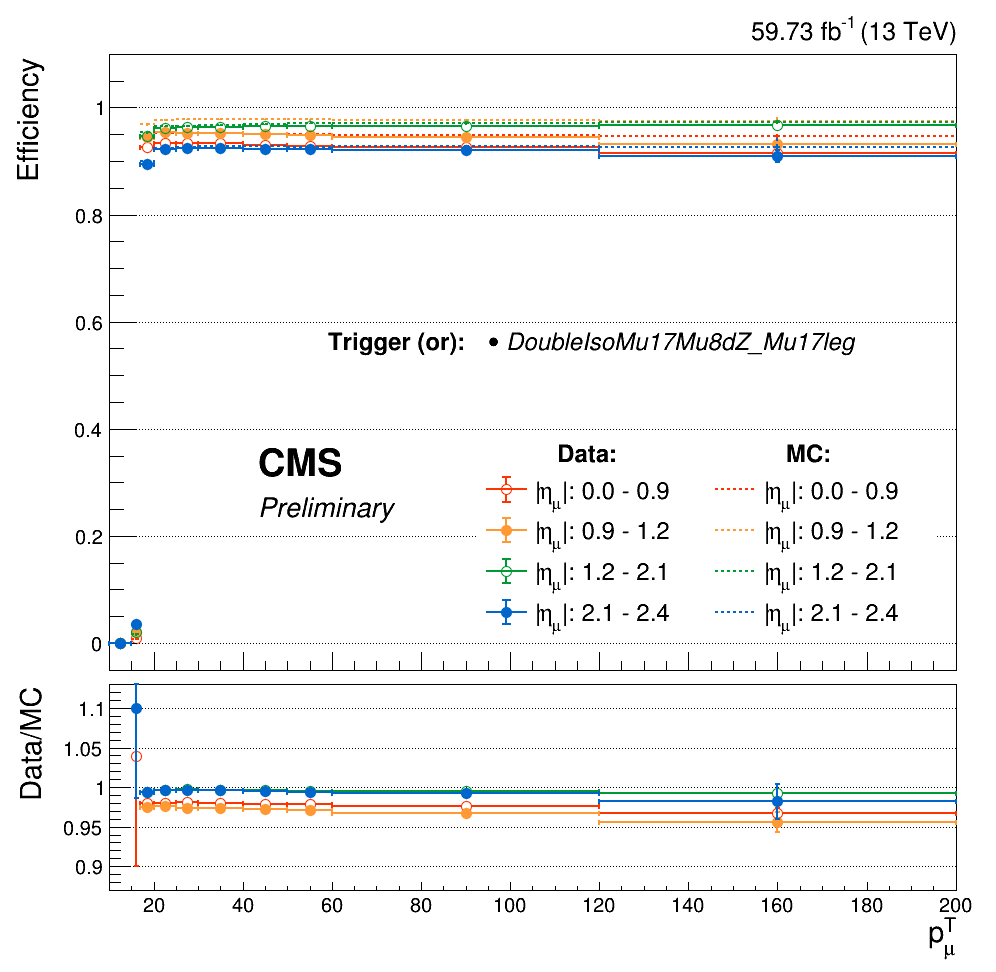
\includegraphics[width=0.30\textwidth]{fig/SFs/sf1D_year2018_leg1.png}
		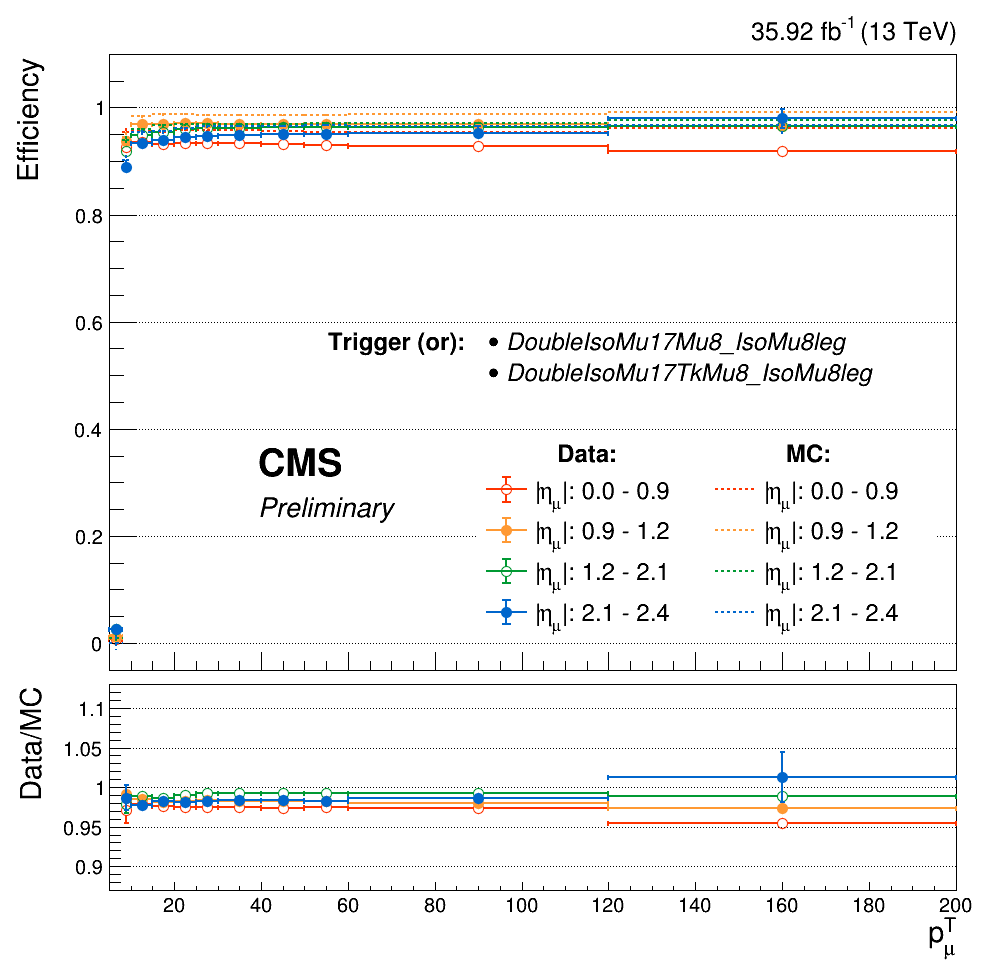
\includegraphics[width=0.30\textwidth]{fig/SFs/sf1D_year2016_leg2.png}
		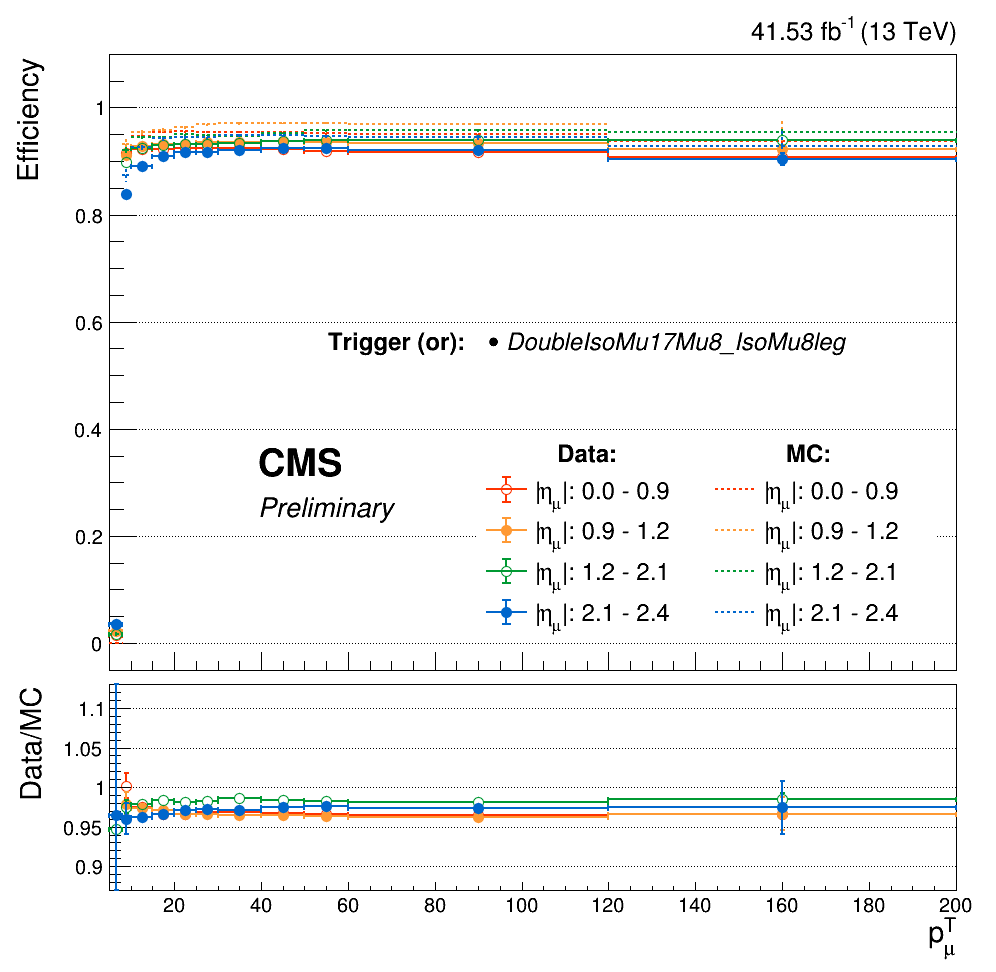
\includegraphics[width=0.30\textwidth]{fig/SFs/sf1D_year2017_leg2.png}
		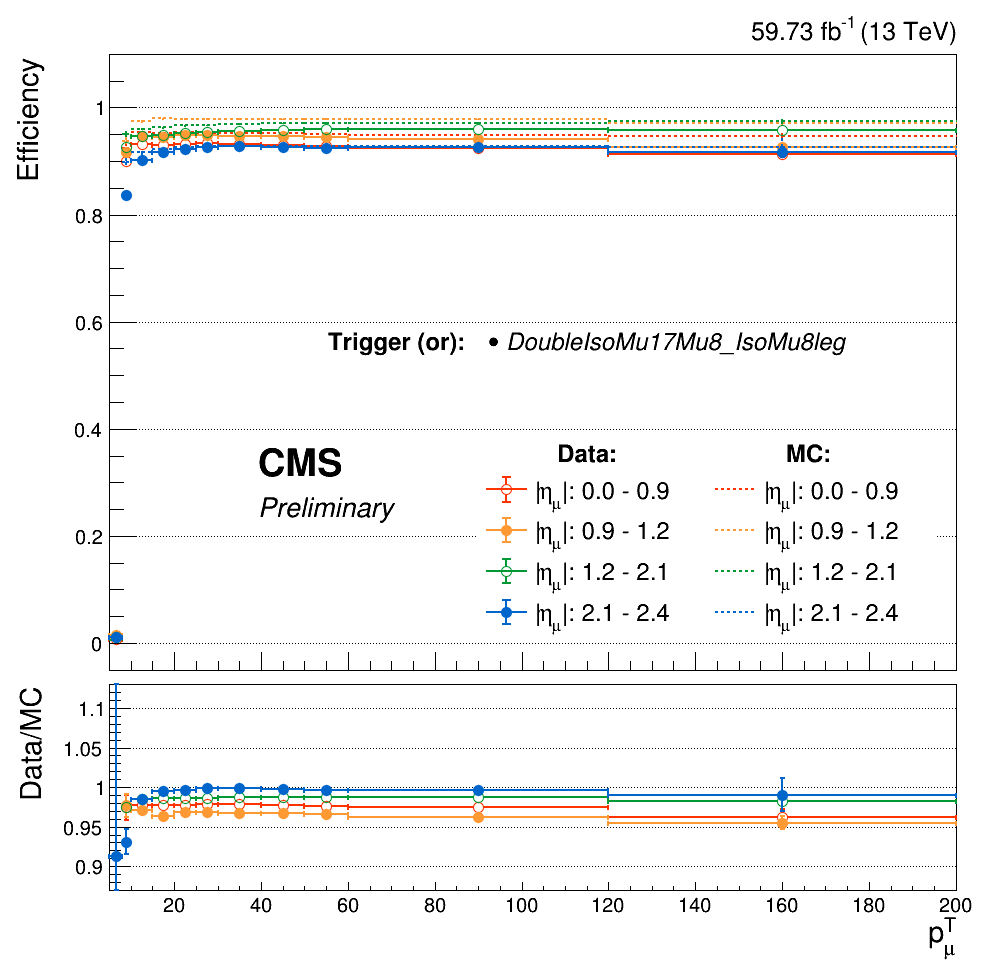
\includegraphics[width=0.30\textwidth]{fig/SFs/sf1D_year2018_leg2.png}
	\end{center}
	\caption{Efficiency measurements for each leg of the double muon trigger in 2016 (left), 2017 (center), and 2018 (right). The upper (lower) plots correspond to the 
	leading (subleading) trigger leg.}
	\label{fig:mu_trig_SF}
\end{figure}

\section{Photon Selection}
Photons are identified using a BDT discriminant (photon MVA ID) trained on $\PGg$+jets simulation in order to distinguish real photons from jets misreconstructed as photons. 
The features used for the BDT training include supercluster kinematics, isolation variables, and shower shape variables~\cite{EGM:PhotonID}. 
To reject electrons faking photons, a conversion-safe electron veto is also applied. In order to improve agreement between simulation and data for the photon MVA ID, shower 
shape corrections are taken from the CMS $\PH\to\PGg\PGg$ analysis of the same data set~\cite{CMS:2021kom} and applied to simulated events. 
The photon MVA ID is then reevaluated after these corrections. We correct the following features: $R_{9}^{5x5}$, defined as the ratio of energy in
the 5x5 array of ECAL crystals to the supercluster energy; $S_{4}$, defined as the ratio of the maximum energy 2x2 array to the energy of 
the 5x5 array; the energy weighted shower widths $\sigma_{\eta}$ and $\sigma_{\phi}$; the energy weighted widths by crystal index 
$\sigma_{i\eta i\eta}$ and $\sigma_{i\eta i\phi}$; photon isolation, charged isolation with respect to the primary vertex, 
and charged isolation with respect to the worst vertex choice. The validity of the shower shape corrections is checked using tag 
and probe procedures for $\PZ\to\epem$ events where the probe electron mimics a photon and $\PZ\to\mpmm$
events with an FSR photon. Comparisons of the agreement between uncorrected and corrected simulation with data for the photon MVA ID are shown in 
Fig. \ref{fig:photon_mva_correction}. Similar plots for individual shower shape features can be found in Appendix \ref{sec:shower_shape}. 

\begin{figure}[tb]
	\begin{center}
		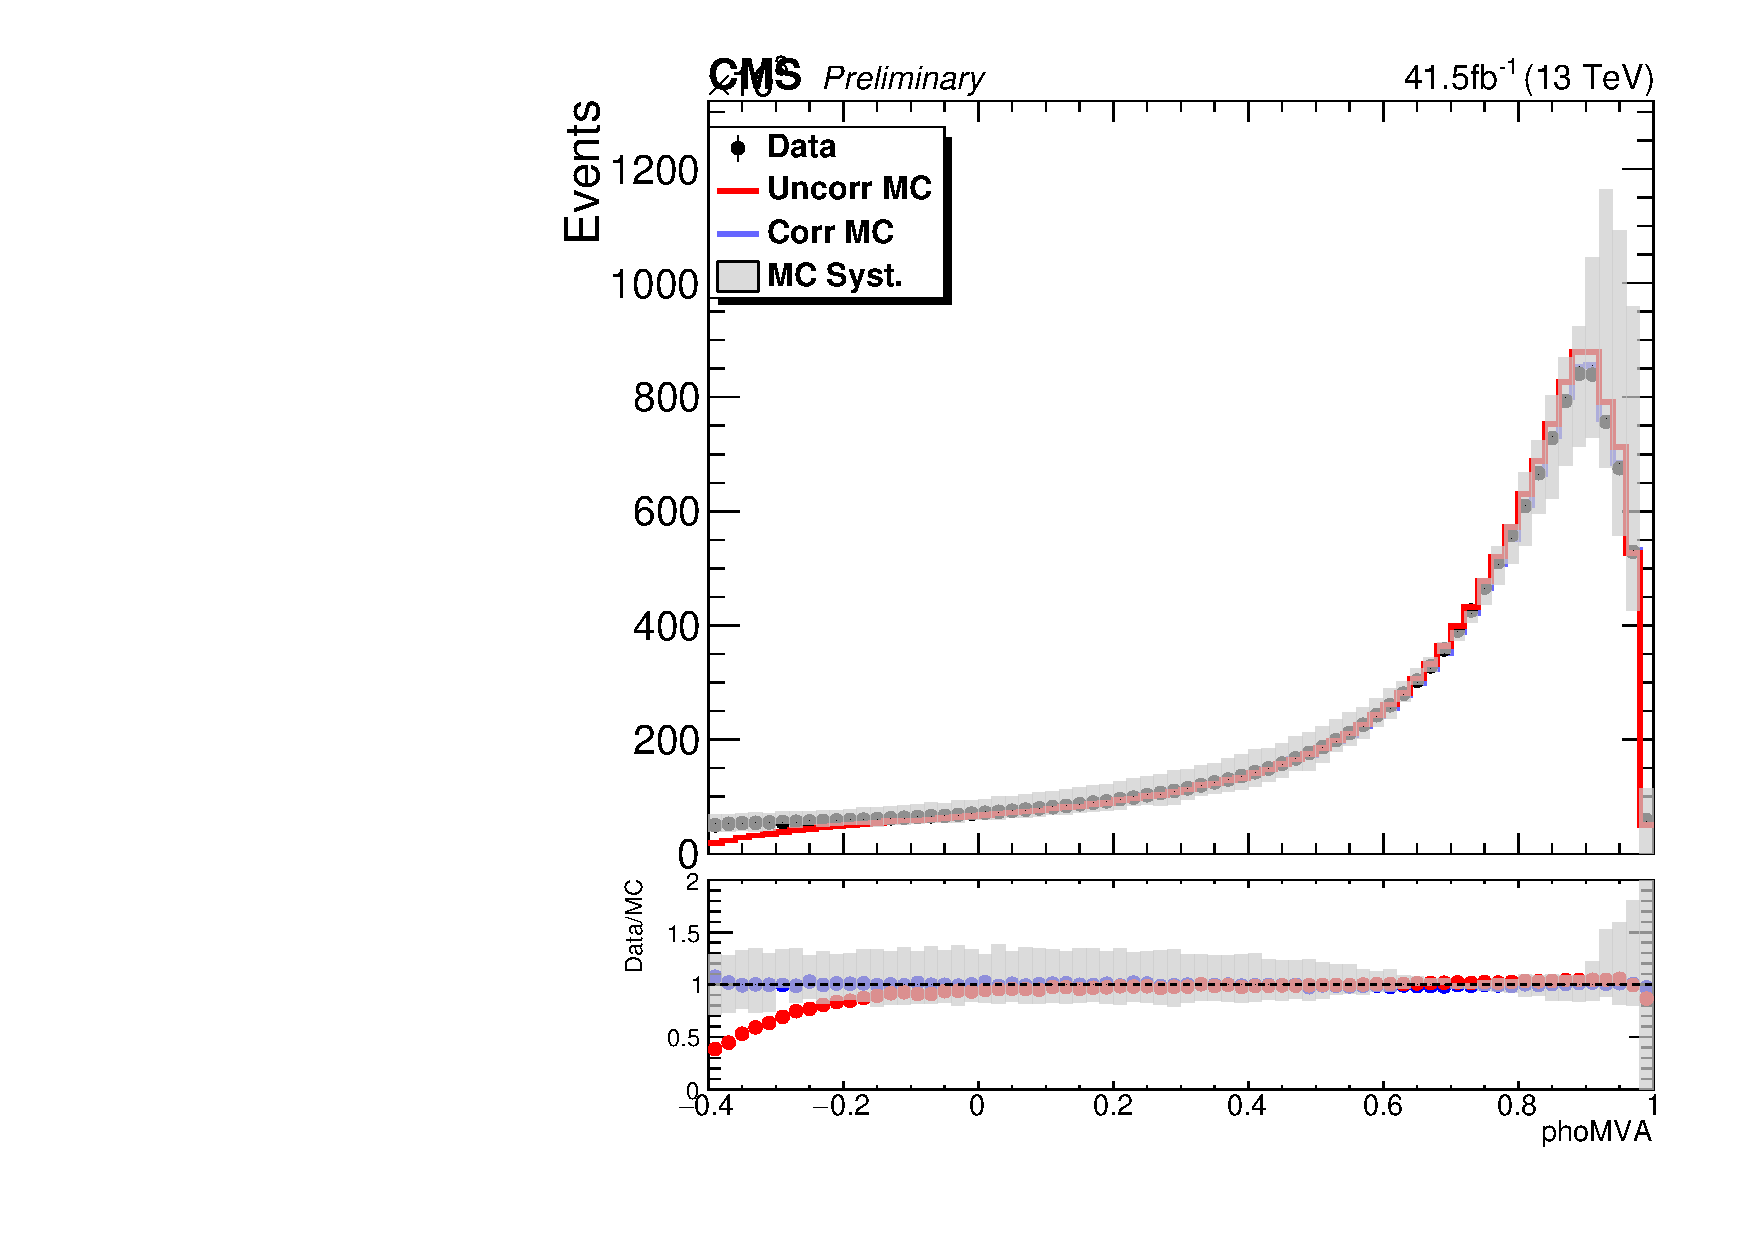
\includegraphics[width=0.35\textwidth]{fig/ss_corr/phoMVA_17_EB_Z.pdf}
		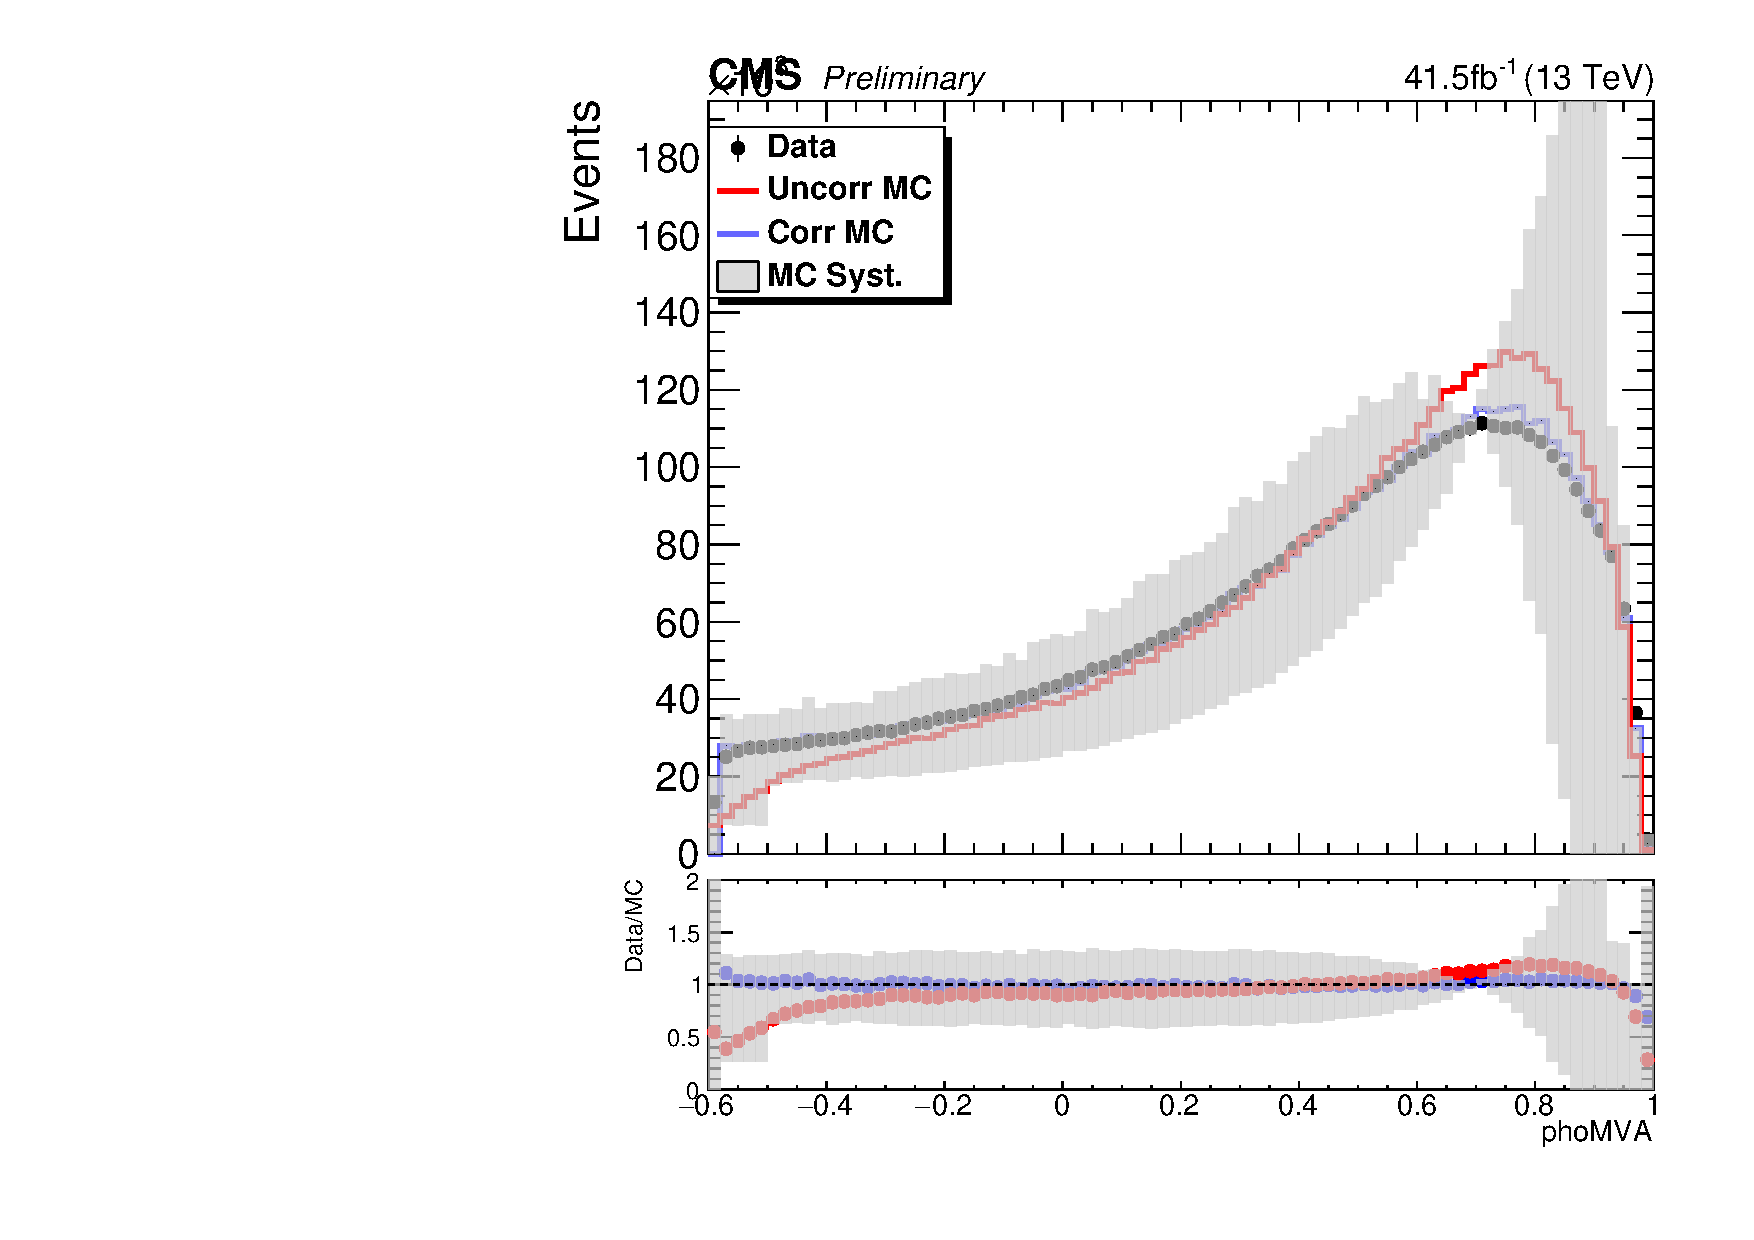
\includegraphics[width=0.35\textwidth]{fig/ss_corr/phoMVA_17_EE_Z.pdf}
		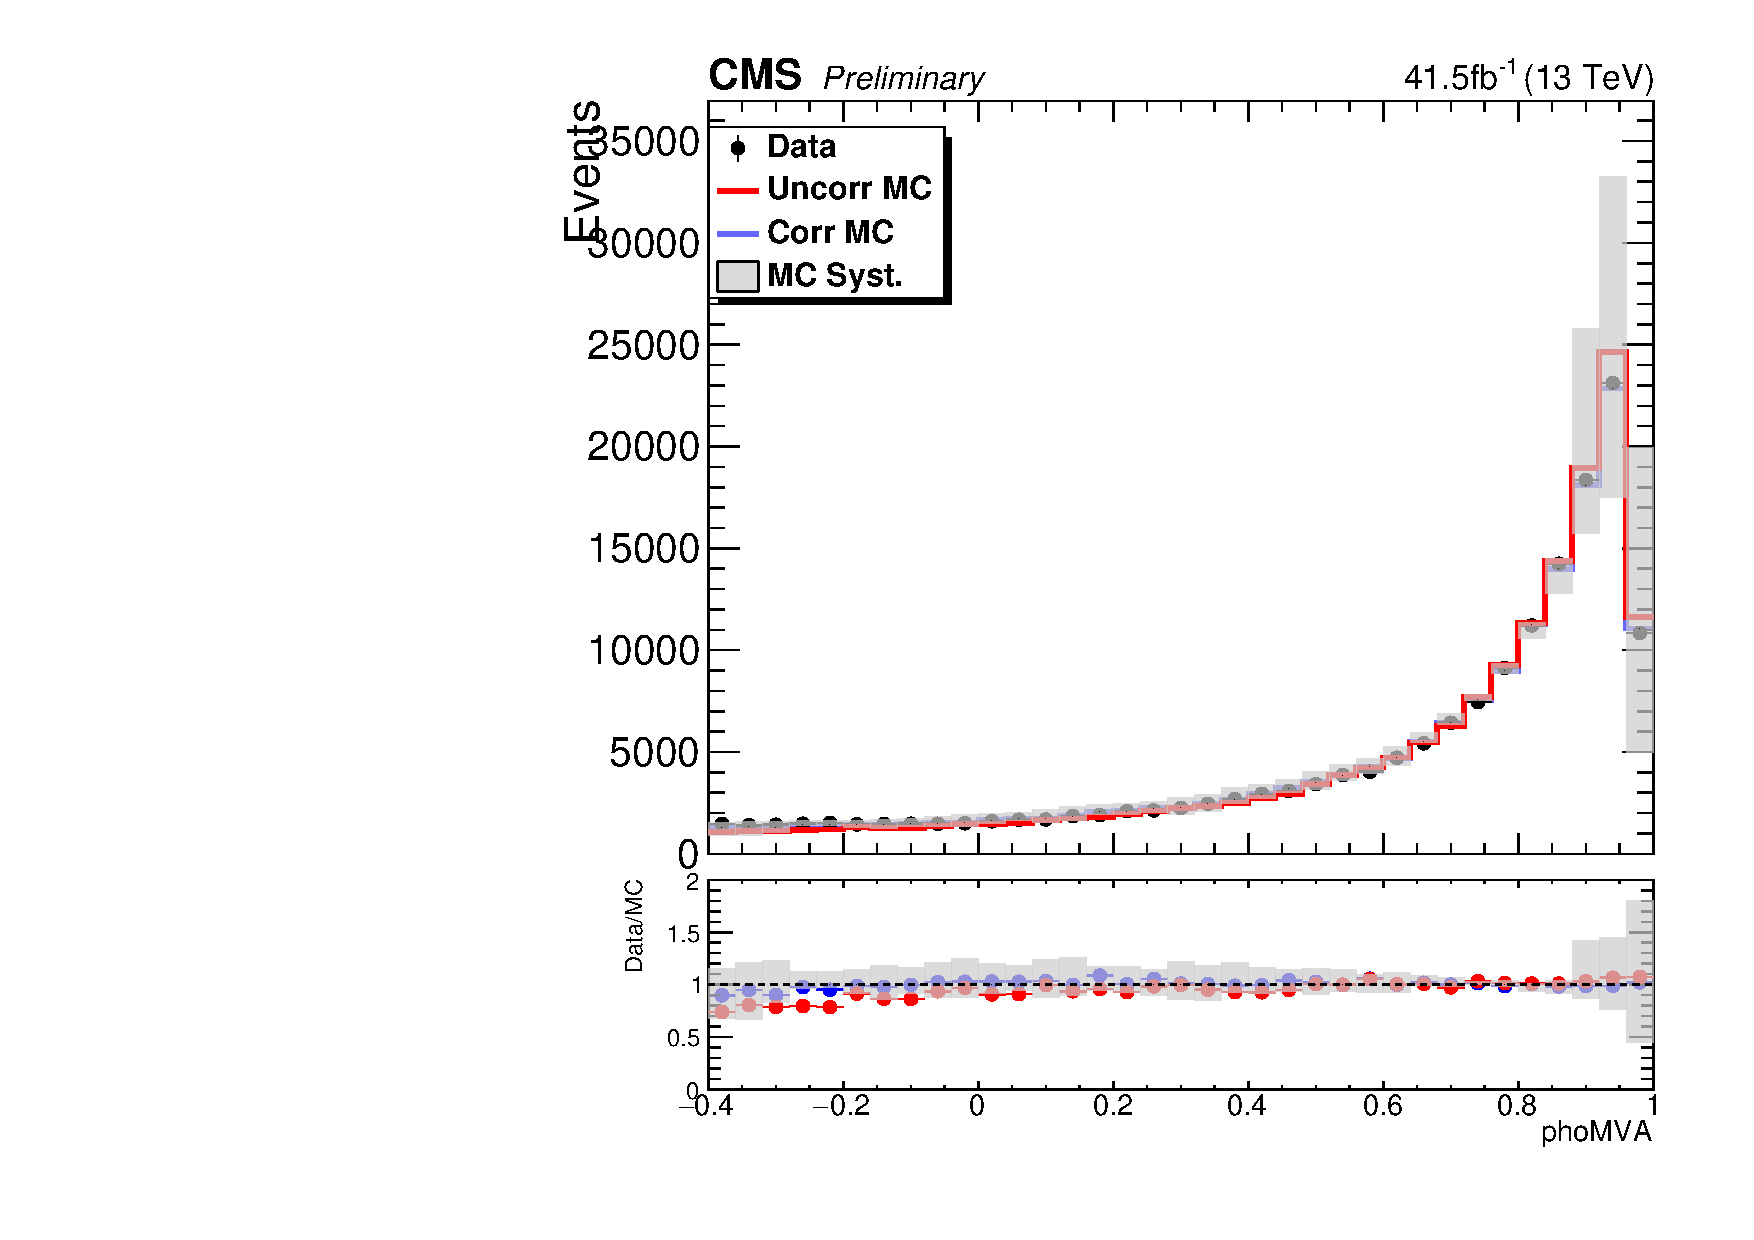
\includegraphics[width=0.35\textwidth]{fig/ss_corr/phoMVA_17_EB_Z_mmg.pdf}
		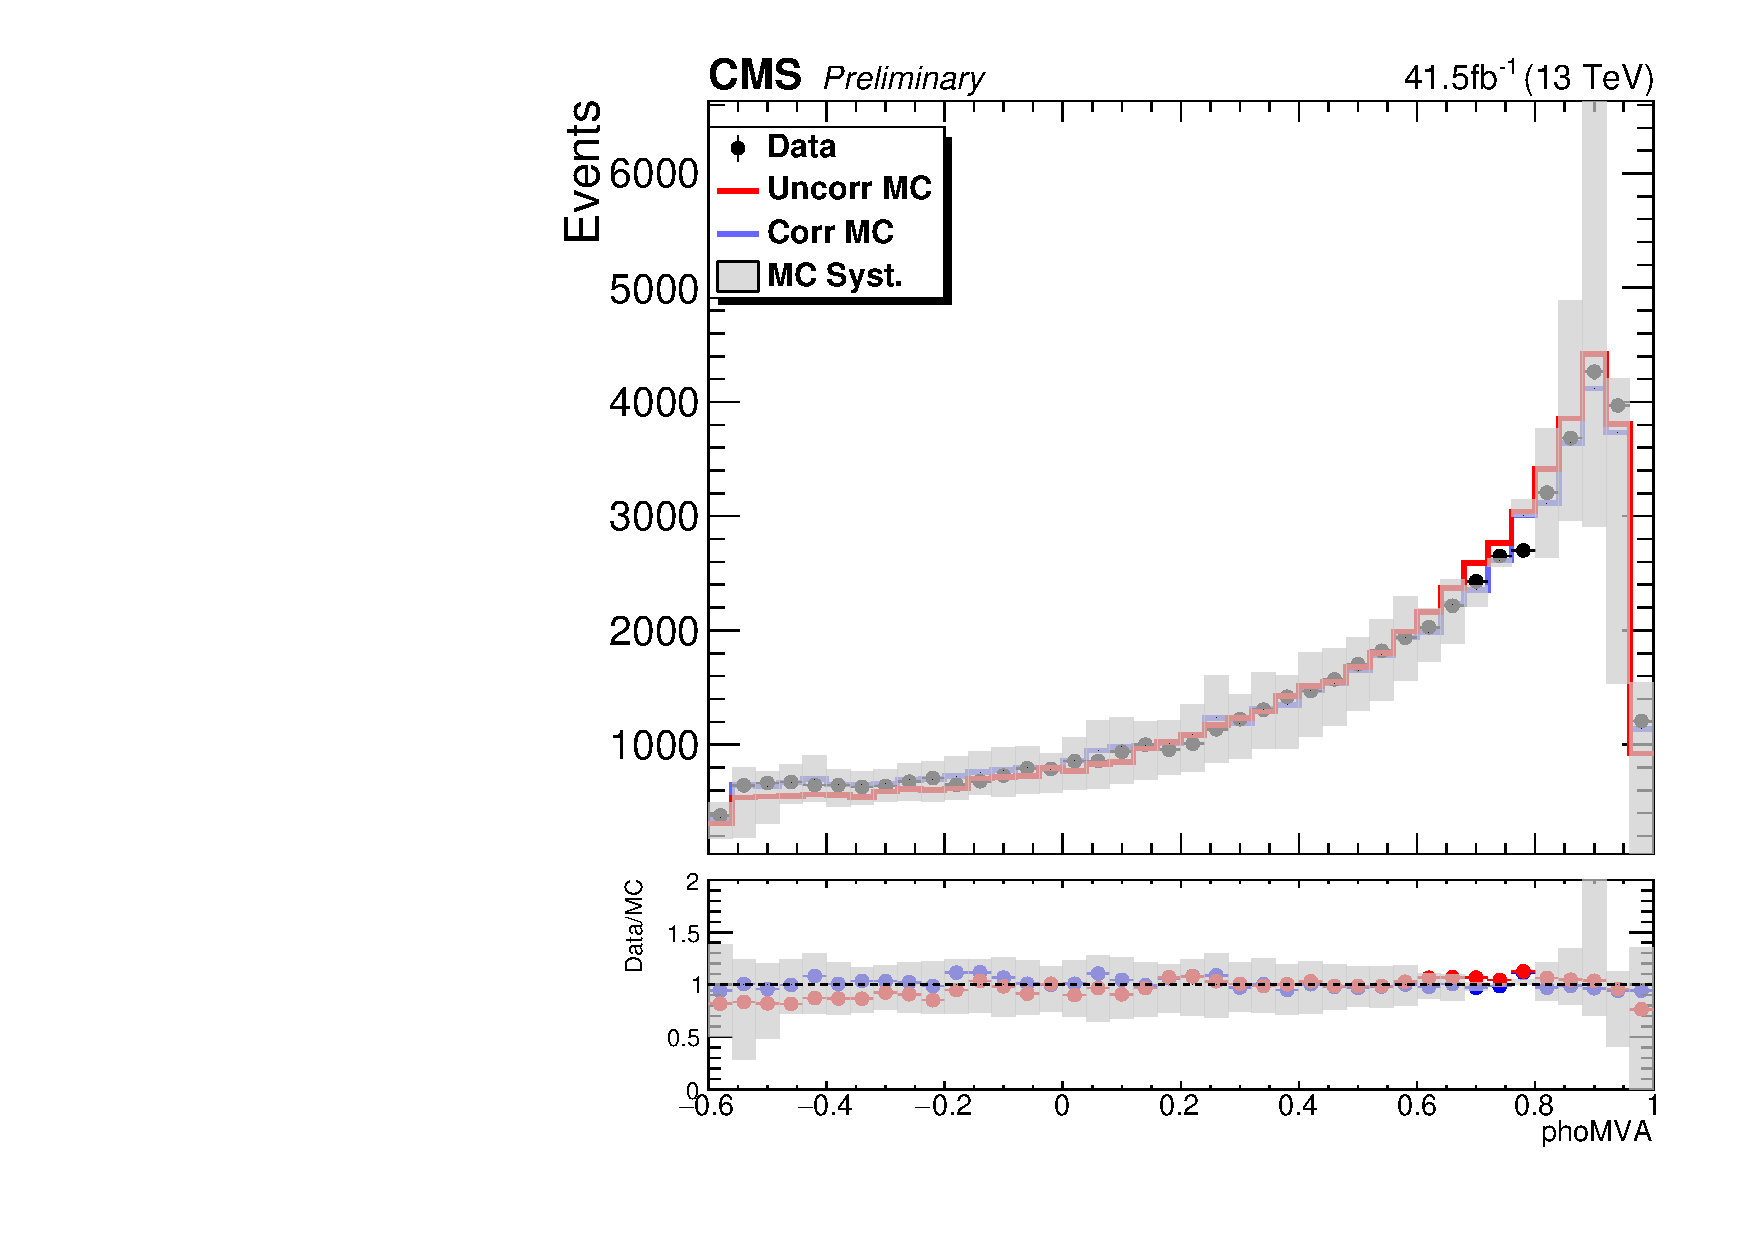
\includegraphics[width=0.35\textwidth]{fig/ss_corr/phoMVA_17_EE_Z_mmg.pdf}
	\end{center}
	\caption{Comparison of simulation with 2017 data for the photon MVA ID before and after shower shape corrections are applied to the simulation. The plots on the left (right) correspond to the barrel and endcap regions, and the upper (lower) plots correspond to $\PZ\to\epem$ ($\PZ\to\mpmm+\PGg$) events.}
	\label{fig:photon_mva_correction}
\end{figure}

Based on the corrected photon MVA ID, 90\% signal efficiency working point (WP) cuts for barrel and endcap photons 
are determined for the \hzg{} analysis. The WPs are defined based on real photons from $\Z\gamma$ simulation, and correspond 
to photon MVA ID scores greater than -0.4 (-0.59) for barrel (endcap) photons. A comparison of these WPs with the general CMS 90\% efficiency WPs, 
plotted on the receiver operator characteristic (ROC) curve for $\PZ\gamma$ (signal) and $\PZ$+jets (background)
simulation, is shown in Fig. \ref{fig:photon_mva_roc}. The efficiency of the photon MVA ID is measured with $\PZ\to\epem$ data
using a tag and probe technique. The tag electron must pass the single electron trigger with \pt threshold 27 (32) GeV in 
2016 (2017 and 2018), pass a tight cut-based identification, have \pt $>$ 30 (35) GeV for 2016 (2017 and 2018), and have $|\eta| < 2.5$. The 
probe electron must pass the corrected photon MVA ID. The corresponding SFs, measured and 
applied in bins of \pt and supercluster $\eta$, are shown in Fig. \ref{fig:photon_id_sf}. The efficiencies and SFs for the conversion-safe 
electron veto are measured by CMS using $\PZ\to\mpmm$ events with an FSR photon and are applied in the \hzg{} analysis. 
These SFs are cataloged in Table \ref{tab:eveto_sf}. 

\begin{figure}[tb]
	\begin{center}
		\includegraphics[width=0.75\textwidth]{fig/selection/photon_ID_ROC.png}
	\end{center}
	\caption{ROC}
	\label{fig:photon_mva_roc}
\end{figure}

\begin{figure}[tb]
	\begin{center}
		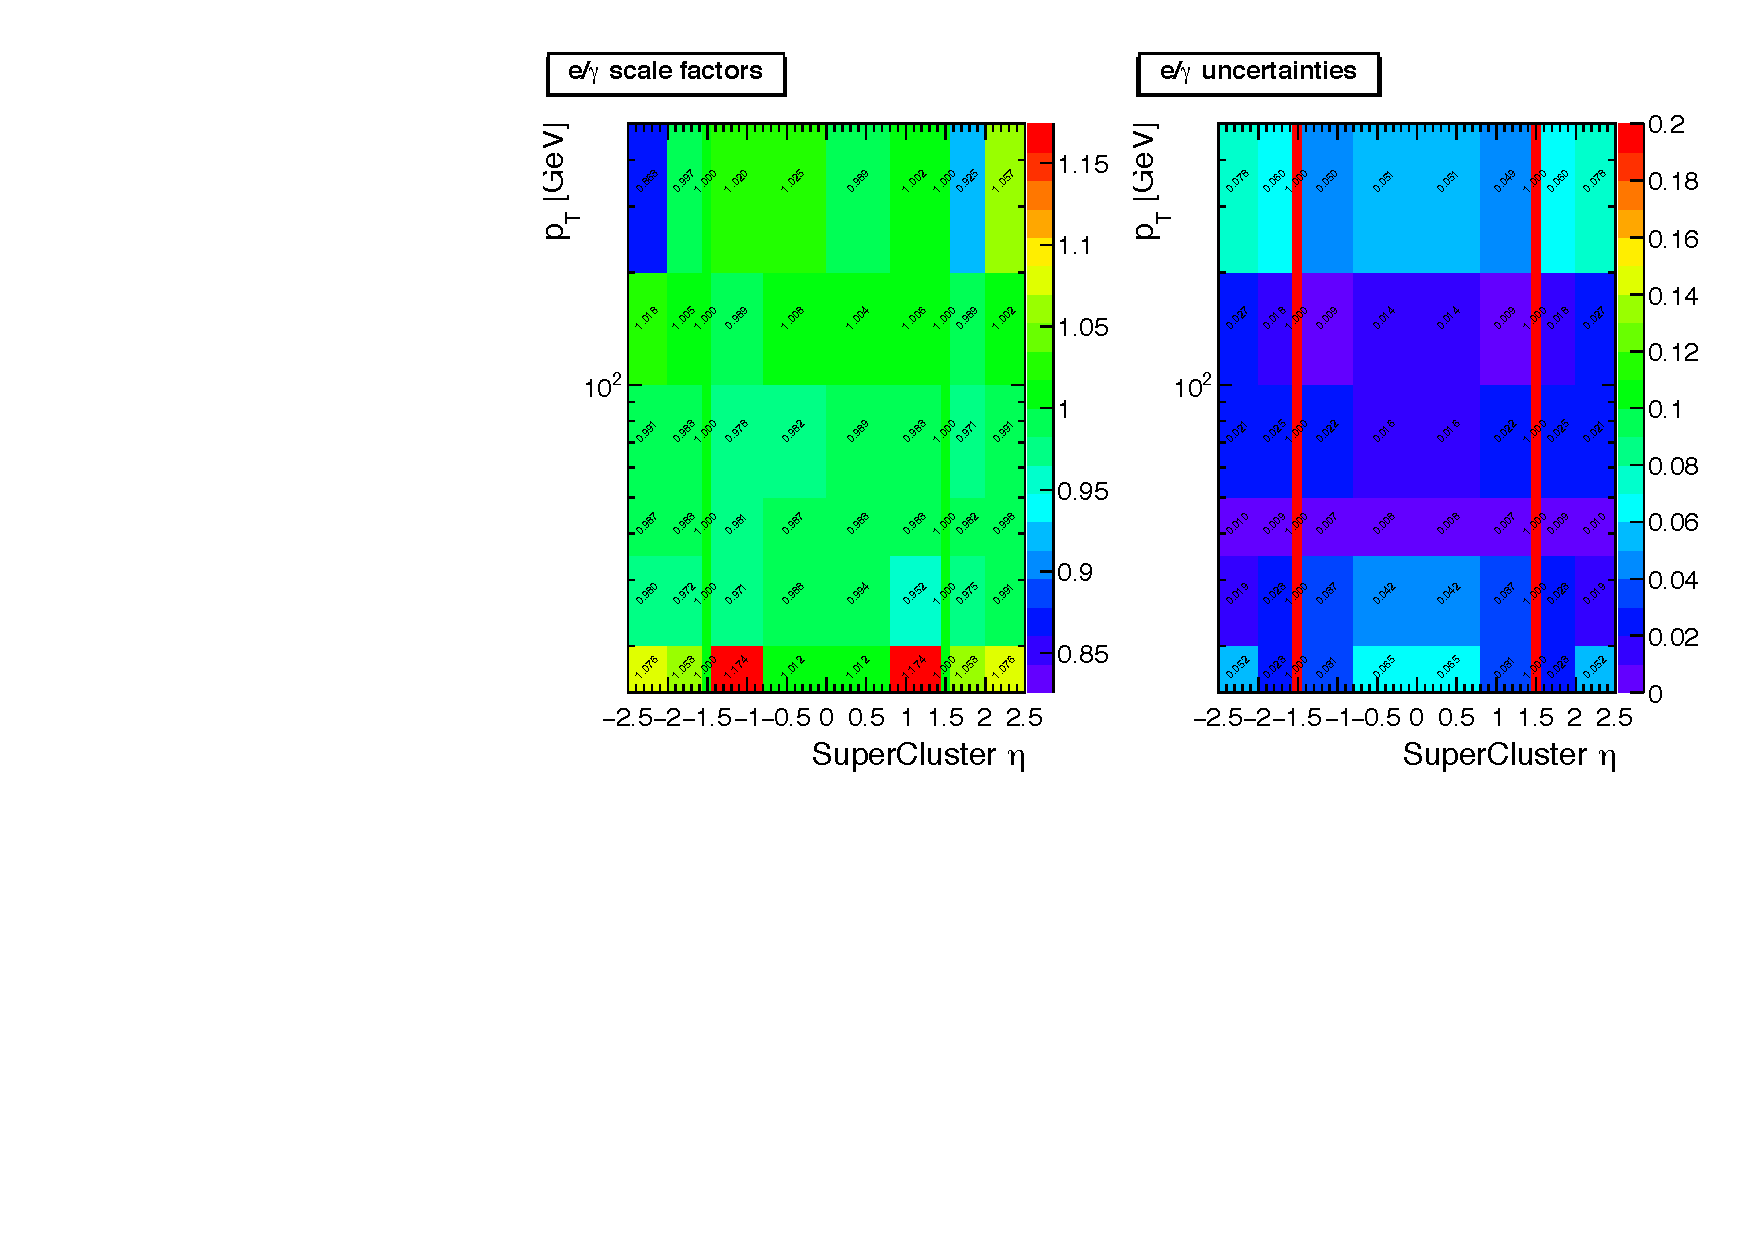
\includegraphics[width=0.7\textwidth]{fig/SFs/2016_ID_pho_2D.pdf}
		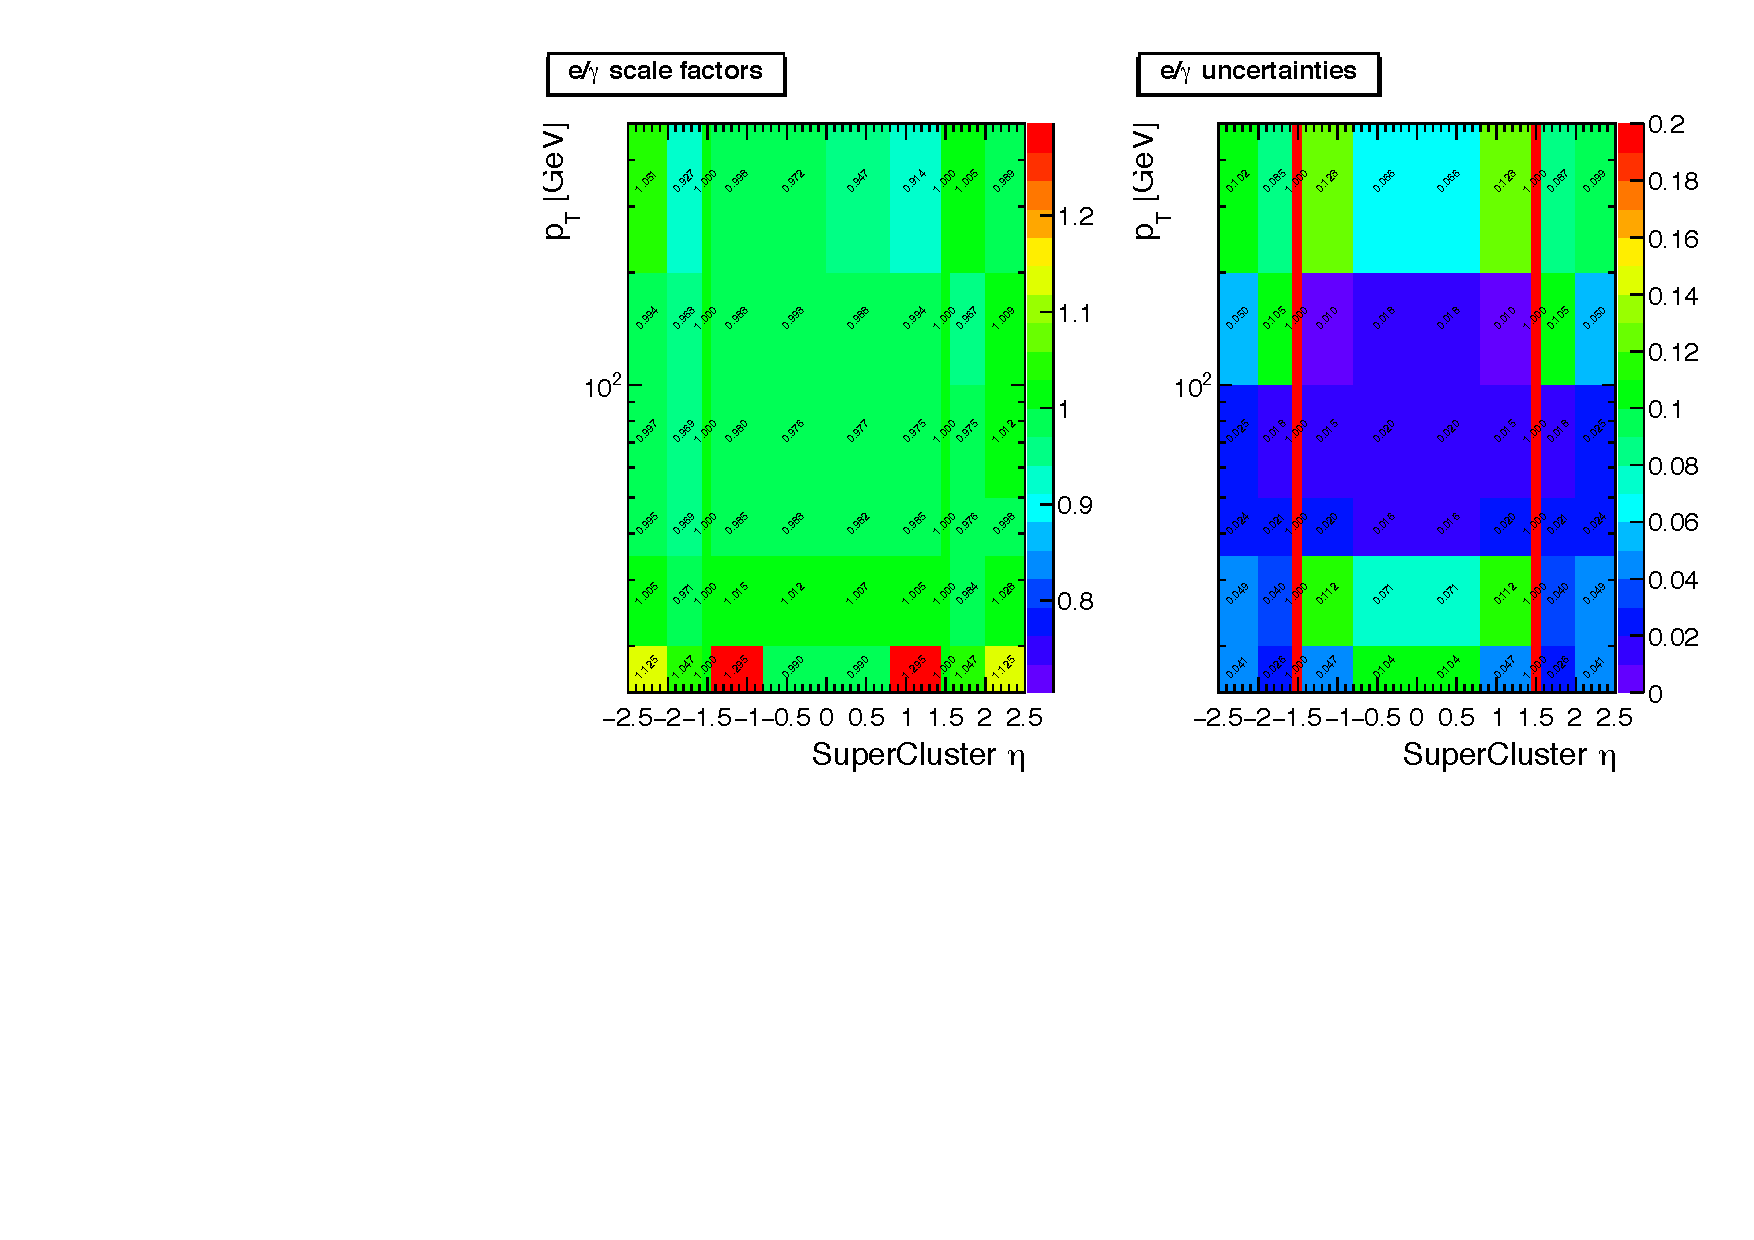
\includegraphics[width=0.7\textwidth]{fig/SFs/2017_ID_pho_2D.pdf}
		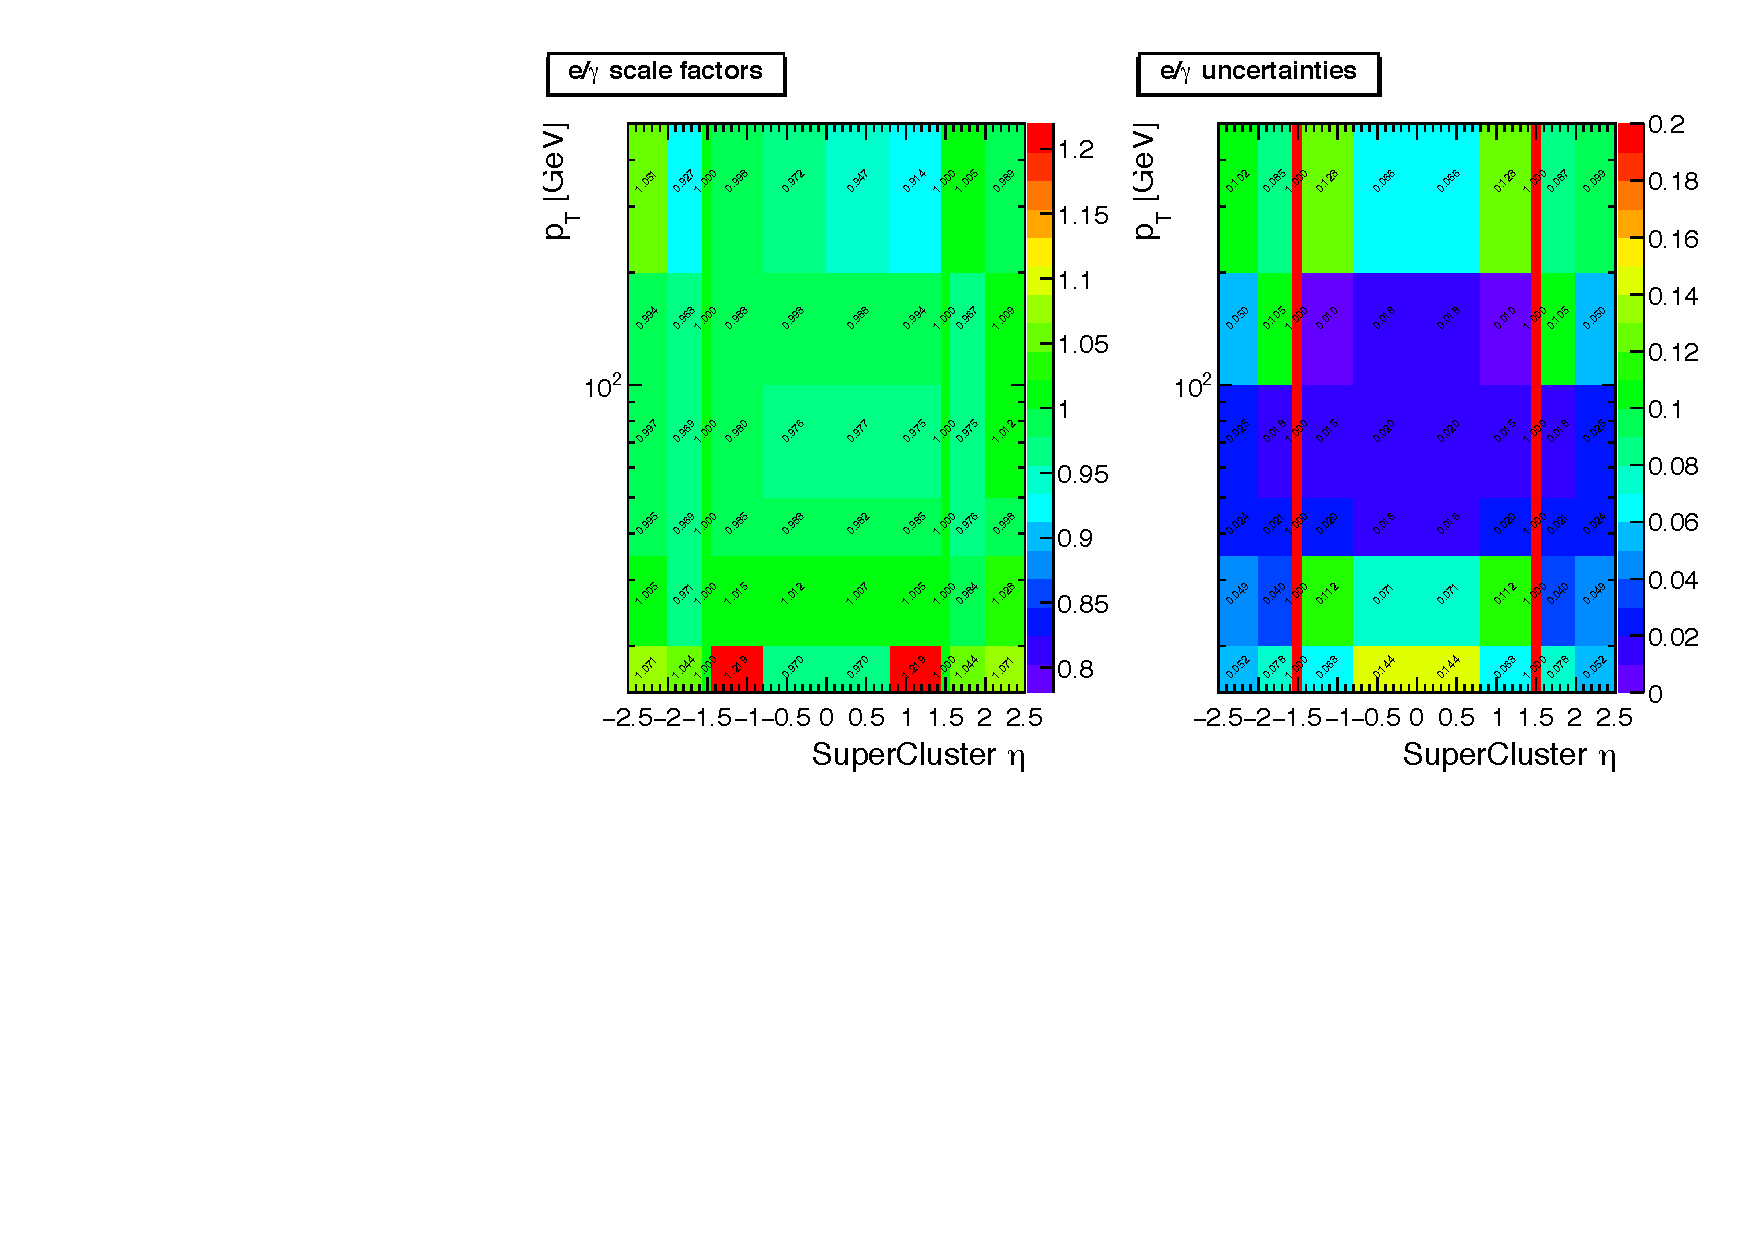
\includegraphics[width=0.7\textwidth]{fig/SFs/2018_ID_pho_2D.pdf}
	\end{center}
	\caption{Photon MVA ID efficiency SFs.}
	\label{fig:photon_id_sf}
\end{figure}

\clearpage

\section{Electron Selection}
Electrons are identified using a boosted decision tree multivariate (MVA) discriminator trained on Drell-Yan plus jets simulation 
with prompt electrons matched to generator-level objects as signal and unmatched and non-prompt electrons as background. The features 
used in the training include \pt, supercluster $\eta$, shower shape variables, ratio of hadronic to electromagnetic energy, track and 
pixel hit variables, and isolation variables [REF]. These features are sensitive to bremsstrahlung along the electron trajectory, 
momentum-energy matching between electron trajectory and ECAL cluster, shower shape, and electrons from photon conversions.
Since isolation features are included in the training of the discriminator, there is no need for separate isolation cuts. 
Electrons pass the identification requirement of the \hzg analysis if their discriminator score is higher than a loose WP
value, corresponding to 98\% signal efficiency. In addition to the MVA cut, electrons must have $|d_{xy}| < 0.5$ cm and $|d_{z}| < 1$ cm
with respect to the primary vertex. Electrons with \pt $\leq$ 7 GeV are rejected. 

Electron identification efficiencies and scale factors are measured using a tag and probe method on dielectron events near the 
Z boson peak. These electrons must pass the single electron trigger with a \pt threshold of 27 (32) GeV for 2016 (2017/2018) data. 
The dielectron mass must be between 60 and 120 GeV. The tag electron must pass a tight cut-based electron identification and have 
\pt $>$ 30 (35) GeV for 2016 (2017) and $|\eta|$ < 2.5. The probe electron must pass the loose MVA identification cut and associated 
impact parameter and \pt cuts described above. Identification efficiencies and scale factors are measured and applied in bins of 
\pt and supercluster $\eta$. The scale factors for each data-taking year are shown in Figures [FIGS]. 

\section{Muon Selection}
A loose cut-based muon identification is used in the analysis. This identification was originally developed by the \hzz 
analysis [REF] and is well-suited for \hzg due to the similarity of the multiple, potentially soft, muons in the final state. 
All muons are first required to pass a set of common cuts, followed by a separate set of cuts for high \pt (greater than 200 GeV) 
and low \pt muons. All muons must satisfy \pt $>$ 5 GeV, $|\eta| < 2.4$, $|d_{xy}| < 0.5$ cm, and $|d_{z}| < 1$ cm, where $d_{xy}$ and 
$d_{z}$ are impact parameters defined with respect to the primary vertex of the interaction using the best muon track. 
Additionally, the three dimensional impact parameter (analogously defined) must have a magnitude less than four times its uncertainty.
Muons must either be reconstructed as global muons or tracker muons. Muons with standalone tracks (tracks only in the muon system) are
rejected. Muons must pass a particle flow-based isolation requirement, where the relative particle flow isolation 
within a $\Delta R = 0.3$ cone is defined as 
\begin{equation}
\label{eqn:pfiso}
	\mathcal{I} \equiv \Big( \sum p_{T}^\text{charged} + \max\big[ 0, \sum p_{T}^\text{neutral} +\sum p_{T}^{\gamma} - p_{T}^\mathrm{PU}(\ell) \big] \Big) / p_{T}^{\ell}.
\end{equation}
Muons must satisfy $\mathcal{I} < 0.35$. 

For muons with \pt $<$ 200 GeV, muons satisfying the common requirements and identified by the particle flow identification
algorithm are selected. For muons with \pt $>$ 200 GeV, muons are selected if they pass the particle flow identification or if they pass
a set of high-$p_{T}$ requirements. These requirements are the following: the muon must be matched to segments in at least two muon 
stations; satisfy $\frac{p_{T}}{\sigma_{p_{T}}} < 0.3$, $|d_{xy}| < 0.2$ cm, $|d_{z}| < 0.5$ cm, have at least one pixel hit, and have 
tracker hits in at least six tracker layers.

In 2016, data-taking was affected by a problem in which the level one trigger sent only one candidate per 60$^{\circ}$ sector instead 
of up to three [REF?]. As a result, when two muons in the same endcap had a low $\Delta \phi$ separation, only one would fire the 
trigger. To account for this, 2016 data events containing identified muons with $\Delta \phi < 70^{\circ}$ in the same endcap region 
are rejected. 

Identification efficiencies and scale factors corresponding to the muon identification above are measured and provided by the 
\hzz analysis working group, and are shown in Figure [FIG].  

\section{Jet Selection}
Jets are selected in order to categorize events coming from potential VBF Higgs production, but no jet multiplicity requirement is present 
for the \hzg selection. In fact, the majority of simulation and data events selected in the analysis have no jets. However, identifying 
and selecting jets to categorize VBF events can still significantly improve the sensitivity of the search. Jets are required to pass 
a loose cut-based identification in 2016 and a tight cut-based identification in 2017 and 2018. These sets of identification cuts are
determined and provided by the JetMET POG. Additionally, jets must satisfy \pt $>$ 30 GeV, $|\eta| < 4.7$, and $\Delta R > 0.4$ with 
respect to each lepton and the photon selected in the analysis. An issue with noise in the ECAL endcap in 2017 caused an artificial 
increase in jet multiplicity in data within a specific kinematic phase space [REF]. To mitigate this, jets are rejected if they have 
raw \pt $<$ 50 GeV and $2.65 < |\eta| < 3.139$. This cut reduces the efficiency to reconstruct dijet pairs by 12\% in the specified 
region. To tag VBF events, we are interested in dijet pairs. To this end, if there are more than two jets satisfying the above criteria, 
only the two jets with highest \pt are selected. 

\section{Object Corrections}
Several standard corrections are applied to the physics objects selected in the analysis. Rochester muon momentum scale and resolution 
corrections are applied to both data and simulation [REF]. Energy and momentum scale and resolution corrections for electrons 
and photons are provided by the EGamma POG and applied in the analysis. Jet momentum scale and resolution correctors are provided by 
the JetMET POG and applied in the analysis. 

An additional muon momentum correction is obtained using an FSR photon recovery procedure, and is based on the procedure used by the \hzz 
analysis [REF]. FSR photons are not considered during the standard CMS muon reconstruction. As the \pt of FSR photons from radiating 
muons is generally very low, particle flow photons are considered, in contrast with the fully reconstructed photons used in the main 
analysis selection. A particle flow photon must pass a set of cuts in order to be identified as an FSR photon associated with one of the 
muons selected by the analysis. The photon must have \pt $>$ 2 GeV, $|\eta|<2.4$, and relative particle flow isolation less than 1.8. 
It must also satisfy $\Delta R(\gamma, \mu)/p_{T,\gamma}^{2} < 0.012$ and $\Delta R(\gamma, \mu) < 0.4$. If multiple particle flow 
photons pass these requirements, the photon with the smallest $\Delta R(\gamma, \mu)/p_{T,\gamma}^{2} < 0.012$ is chosen. 
Then, the four momentum of the FSR photon is added back to the four momentum of the muon, and the muon kinematics reevaluated. 
In simulation, we find that the selected FSR photon matches the generator level FSR photon with 93\% efficiency. 
Figure [FIG] shows the dilepton and three body 
invariant mass among FSR photon-containing signal events with and without applying the FSR recovery correction.
The procedure yields a 1\% improvement on the three body mass resolution in the muon channel.

\section{Event Selection}
Events are required to have at least one good primary vertex
with a reconstructed longitudinal position within 24\,{cm} of the
geometric center of the detector and a transverse position within
2\,{cm} of the nominal beam collision point. The vertex with the largest value of summed physics-object
$p_{T}^2$ is taken to be the primary interaction vertex. The physics objects used in this calculation are derived from 
information obtained from the charged-particle tracking detectors only. These objects include jets reconstructed by 
clustering charged particle tracks; the associated missing transverse momentum, defined as the negative vector sum of the \pt of 
those jets.

Events with two same-flavor opposite sign leptons (e or $\mu$) and a photon are selected. The leading muon (electron) is required to have 
\pt greater than 25 (20) GeV, and the trailing lepton must have \pt greater than 15 (10) GeV. Electrons (muons) must have $|\eta|$ 
less than 2.5 (2.4). The photon must have \pt greater than 15 GeV and must satisfy $0 < |\eta| < 1.4442$ or $1.566 < |\eta| < 2.5$. 
This avoids the calorimeter transition region, in which photon reconstruction is more difficult. The invariant mass of the dilepton 
system is required to be greater than 50 GeV. In events with multiple dilepton pairs, the pair with mass closest to the nominal 
Z boson mass [REF] is selected. 

Events are required to have a photon satisfying $p_{T}^{\gamma}/m_{\ell\ell\gamma} > 0.14$, which suppresses the Z plus jets 
background without significantly reducing signal efficiency and without significantly shaping the three body mass spectrum.
Each lepton must have $\Delta R > 0.4$ with respect to the photon. To reject events with final-state radiation from 
Drell-Yan processes, we require $m_{\ell\ell\gamma} + m_{\ell\ell} > 185$ GeV. Finally, the three body mass is required to 
satisfy $105 < m_{\ell\ell\gamma} < 170$ GeV. 

\section{Kinematic Fit}
A kinematic fit technique is used to improve the dilepton mass resolution. This constrains the dilepton mass based on the true 
Z boson lineshape while accounting for the known detector resolution. The position information of the leptons has a negligible impact
on the fit, so only the lepton transverse momenta and dilepton mass are included in the fit. The procedure is based on previous
studies by the \hzz analysis [REF]. We do not carry out an analogous kinematic fit for the $m_{\ell\ell\gamma}$ invariant 
mass in order to avoid any potential bias due to reshaping the mass distribution. The kinematic fit is a maximum likelihood fit 
defined by the likelihood function below: 

\begin{equation}
\begin{aligned}
\mathcal{L}({P_{T}}^{1},{P_{T}}^{2}|{P_{T}}^{reco1},{\sigma_{P_{T}}}^1,{P_{T}}^{reco2},{\sigma_{P_{T}}}^2) \\
=Gauss({P_{T}}^{reco1}|{P_{T}}^{1},{\sigma_{P_{T}}}^1)\cdot Gauss({P_{T}}^{reco2}|{P_{T}}^{2},{\sigma_{P_{T}}}^2)\cdot\mathcal{L}(m_{12}|m_{Z})
\end{aligned}
\end{equation}

Here, $p_{T}^{reco1}$ and $p_{T}^{reco2}$ are the reconstructed transverse momenta of the two leptons, 
$\sigma_{p_{T}}^{1}$ and $\sigma_{p_{T}}^{2}$ are the per-lepton transverse momentum resolutions, 
$p_{T}^{1}$ and $p_{T}^{2}$ are the parameters to optimize, and $m_{12}$ is the invariant mass 
calculated from $p_{T}^{1}$ and $p_{T}^{2}$. $\mathcal{L}(m_{12}|m_{Z})$ is the likelihood given the true Z mass lineshape. 
The outputs of the fit are $p_{T}^{1}$ and $p_{T}^{2}$.
Their uncertainties are saved and used to calculate a per-event uncertainty for the mass measurement.
To optimize this procedure, we determine the true generator level Z lineshape from a gluon-gluon fusion \hzg sample.
Generator level Z lineshapes for the dielectron and dimuon final states are fit with 
a single-sided Crystal Ball function plus three gaussian functions.
For each event, the likelihood is maximized and the \pt information of the refit leptons is updated. 
Then, the dilepton mass and three body mass are recalculated based on the refit leptons.
The mass distributions for before and after the kinematic fit are shown in Figure [FIG]. The level of improvement in the 
dilepton mass resolution, 
as measured by $\sigma_{eff}$, is shown in in Table \ref{tab:sig_eff_refit}.

\begin{table}[h]
    \begin{center}
    \caption{
        Percent improvement in dilepton and three-body mass resolution (measured by $\sigma_{eff}$) 
        after the kinematic fit.
      }
        \begin{tabular}{|c|cc|cc|}
      \hline
               & \multicolumn{2}{c|}{\textbf{electron channel}}   & \multicolumn{2}{c|}{\textbf{muon channel}}               \\
	  \hline
		&$m_{ee}$&$m_{ee\gamma}$&$m_{\mu\mu}$&$m_{\mu\mu\gamma}$\\\hline
            \textbf{2016} & 20\% & 20\%& 17\% &12\%\\ 
      \hline
            \textbf{2017} & 28\% & 27\%& 21\% &11\%\\ 
      \hline 
            \textbf{2018} & 24\% & 24\%& 20\% &10\% \\ 
      \hline 
    \end{tabular}
    \label{tab:sig_eff_refit}
    \end{center}
\end{table}

We also perform a closure test on the background as shown in Figure [FIG]. The dilepton mass should be constrained,
while the three body mass should not be distorted by the kinematic constraint. Indeed, this is what is observed.
